\documentclass[draft,landscape, 11pt, oneside]{report}
\usepackage[a4paper, left=2cm, right=2cm, top=2.5cm]{geometry}
%\usepackage[T1]{fontenc}
\usepackage{lmodern}
\usepackage{hyperref}
\usepackage{titlesec}
\usepackage{scrextend}
\usepackage{array}
%\usepackage{fontspec}
\usepackage[inline]{showlabels}
%\setmainfont{FiraSans-SemiBold}
\setlength{\parindent}{0pt}
\setlength{\parskip}{1em}
\setlength{\leftmargin}{-4cm}
\setlength{\paperheight}{210mm}
\setlength{\paperwidth}{297mm}
\setlength{\textwidth}{26cm}
\setlength{\footskip}{2.5cm}
\renewcommand{\familydefault}{\sfdefault}

\newenvironment{flowtext}{\addmargin[0cm]{7cm}}{\endaddmargin} % standard text width (reduced for layout)

\title{[DRAFT] User Manual for the GliGli upgraded Prophet 600}
\author{Florian Merz (Editor)}
\pagestyle{myheadings}\markright{[DRAFT] User Manual for the GliGli upgraded Prophet 600}
\makeatletter
\renewcommand\chapter{\pagestyle{myheadings}\markright{[DRAFT] User Manual for the GliGli upgraded Prophet 600}\global\@topnum\z@\@afterindentfalse\secdef\@chapter\@schapter}
\makeatother
\titleformat{\chapter}[display]{\pagebreak\LARGE\bfseries}{}{0.0cm}{}
\titlespacing{\chapter}{0pt}{*0}{*0}
%\titleformat{\section}[display]{\Large\bfseries}{}{0.0cm}{}
\titlespacing{\section}{0pt}{*0}{*0}

\begin{document}

%\maketitle
\tableofcontents


\pagebreak
\chapter{Introduction to the GliGli Prophet 600 Firmware Upgrade}

\begin{flowtext}

\section{What you can expect from the Firmware Upgrade}

The credit of the original idea and implementation of the Prophet 600 firmware upgrade belongs to GliGli\cite{gligli}. He describes his motivation as follows:

\begin{addmargin}[2cm]{1cm}

\textit{I love vintage analog synthesizers, and to be honest, my dream synth would be a Prophet 5, but when I heard what the Prophet 600 was capable of tone wise, I immediately thought its major weaknesses -- the lousy computer part, software envelopes and LFO -- could become its strength with a remake; basically the whole internal synth in voltage-controlled from a nice 14bit DAC, so with a fast modern micro controller, it could become awesome, maybe even better than a Prophet 5!}

\end{addmargin}

The original Sequential Circuits Prophet 600 is run by a Z80 processor. This processor and firmware written for it reach their limits when computing the voltages, scanning user inputs and managing MIDI events making the instrment glitchy and non-responsive. GliGli reversed engineered the original firmware for the Z80 and found that the Z80 can be replaced by a (more) modern Teensy 2.0++ USB programmable microprocessor \cite{teensy}. The Teensy not only fits in to the 2x20 pin standard header but could also be programmed to take the role of Z80 with only slight modifications. In this way the limitations of the original Prophet 600 could be overcome - but more than that, it opened the possibility for new features (which may or may not have been on the feature list of Sequential Circuits). There are various modifications and modern CPU "implants" for some vintage analog synthesizers. One decisive advantage of the Teensy approach to the Prophet 600 is that it is an easy-to-install and non-destructive firmware drop-in replacement\footnote{There are two versions of the Prophet 600. One has the Z80 on a socket. In this case replacement is truly "drop-in". The other version has the Z80 soldered to the circuit board. In this case the Z80 needs to be removed a socket has to be soldered in its place first.}. So it is safe to try it out because one can always remove the Teensy board and restore the Z80 without technical expertise or training.

Developing the software was a major effort with low level functions at the core which deal with setting voltages to the electronic components, processing clock alignment, MIDI implementation, decoding the user inputs from dials, buttons and the keyboard and last but not least the "musical" coding of envelopes, modulations and sequencing functions. Many people have contributed, many out of curiosity and passion for synthesizers, most out of excitement that such a project could not only be conjured up but also be implemented and brought to life. The hardware of the Prophet 600 certainly justifies the effort: other than many DCO synths of the time the Prophet 600 is a 6 voice analog synthesizer driven by 12 voltage controlled oscillators (VCOs) and 24db low pass filters, all implemented using the famous Curtis chips\cite{curtis}. Furthermore, the hardware provides hard sync, ring modulation and modulation of cut-off by VCO. It is very versatile.

The following is a compact summary of the improved and the  new features which the upgraded Prophet 600 provides on this hardware. The manual refers to version 2.2 and differences between versions are marked or commented in the text. 

\begin{itemize}
  \setlength\itemsep{0cm}
  \item{General features}
  \subitem Greater resolution of many of the sound parameters with an improved refresh rate that is making the instrument much more responsive
  \subitem Faster and smoother ADSR envelopes with support two speed regimes (slow, fast) and two shapes (linear, exponential)
  \subitem positive and negative envelope amount settings for filter and poly-mod
  \subitem A new LFO function generator with a wider frequency range from one cycle every 20 seconds to about 60Hz
  \subitem Assignable, Random And Up/Down Arpeggiator sync-able to MIDI clock
  \subitem Multiple note assignment modes including last/low/high note priority
  \subitem Full MIDI In control including amplitude and filter velocity sensitivity with an external keyboard controller, continuous Controllers (CC) of all sound parameters, program change (PC) to choose current preset
  \subitem A dedicated vibrato which can be controlled by the modulation wheel, or can start progressively after a fixed amount of time
  \subitem Keyboard mode chord in addition to polyphonic and unison  
  \subitem Four new waveforms in addition to the original triangle and square including sine, random stepped, noise (like on the original Prophet 5, but non-periodic) and sawtooth (ramp up)
  \subitem Mix Overdrive which now allows the output from both oscillators to drive the mix VCAs A and B harder as well as the Curtis 4 pole filter resulting in new sonic possibilities
  \subitem Pitch Wheel interval selection of plus/minus one octave, a whole tone, a minor third and a fifth
  \subitem Pitch Wheel reassignment to the VCF and Volume or off   
  \subitem Modulation wheel intensity setting from Maximum to Medium to Minimum
  \subitem A new and improved tuning procedure
  \subitem Octave, chromatic and free Oscillator course pitch control
  \subitem Debounce feature that prevents unintended re-triggering caused by the old keyboard
  \item Features with version 2.1 RC3
  \subitem Polyphonic step sequencer
  \subitem Per note tuning
  \subitem Support for external CV
  \subitem Improved UI, introducing display of -50...48 range for bipolar dials and center deadband for better handling  
  \subitem VCF limit option
  \subitem Maintenance mode
  \subitem Support for pedal to sustain notes and to hold chords (in unison)
  \subitem On-the-lfly transpose function for arpeggiator and sequencer
  \item Features with version (t.b.d.)
  \subitem A new UI concept in preset mode in which the dials have a pick-me-up behaviour, in order to avoid discontinuous value changes and to make the differences between panel and internal values transparent 
  \subitem Flexible envelope routing allowing the poly-mod to by modulated by either envelope generator
  \subitem Possibility to sync the LFO to the thythm of the arpeggiator or sequencer
  \subitem Continuous spread parameter introducing voice variations in tune and envelopes
  \subitem Better MIDI integration possibilities through new local off mode
  \subitem Improved patch management via MIDI, supporting loading MIDI patch to active controls 
  \subitem Various improvements such as arppegiator / sequencer speed stability and reconciliation of internal and external bend  
  
\end{itemize}

\section{Versions of the firmware upgrade and compatibility}

The first stable version of the Firmware Upgrade was version 2.0 \cite{versiontwo}. An intermediate release (or at least something close to a release) version 2.1 Release Candidate 3 has been available from September 5th 2015 on \cite{gligli}. The current release is version (t.b.d.). 

Upgrading the firmware can be done by SysEx (or directly using the USB port of the Teensy board), see section \ref{fwupgrade}. When upgrading the Prophet 600 patch data and settings are preserved. Note that since this is an open source project different variants of the firmware upgrade have been developed by users. In the main development branch, however, backward compatibility is intended to be ensured. This applies in particular to patches and settings as stored in the Prophet 600 memory or dumped SysEx files. It also applies to the panel overlay which some users have acquired to reflect the (slightly) altered function of some dials. 

\textbf{For users upgrading from version 2.1 RC3}

\textbf{For users upgrading from version 2.0}

\section{Credits and license}

The Firmware Upgrade project has been set up by GliGli as an open source project with a public code repository on GitHub\cite{repository}. 

(this needs to be done)

Despite the fact that many have contributed and have spent considerable time to make this software as useful and consistent as possible and despite the fact that many users continue to enjoy the upgrade, the usage of the software and this documentation are understood to be at the user's own risk.


\end{flowtext}

\chapter{Finding your way around your new  Prophet 600}    

\begin{flowtext}

\section{Display}

The 2 digit 7 segment display is used for different purposes.

\begin{itemize}
  \setlength\itemsep{0cm}
  \item Numeric controls: if the synth is in live mode (see section \ref{uimode}) and the user turns a dial, the display shows the value of the dial. A decimal point between the two digits indicates a negative value. Values range from -50 to 48 (signed parameters) or 0 to 98 (positive parameters). Note that this is a limitation of the display only and that the true resolution of the underlying parameters is higher for many parameters.  
  \item Parameter names and values: additional parameters are "hidden" in menus accessible via the key pad. The chosen parameter name and value are scrolled through the 2 digit display
  \item Messages such as the welcome message (software version) and confirmative messages (e.g. note of completion after a SysEx dump) are also scrolled through the display
  \item During the tuning procedure the current status is shown        
\end{itemize}

\section{Panel control}

(this needs to be done)

\section{Keyboard and performance section}

(this needs to be done)

\section{Key pad and parameter/settings menus}

With the firmware upgrade the Prophet 600 provides additional patch parameters and instrument settings. These are "hidden" in two new menus. The two menus are accessed using the \textbf{Number Pad} in the following way. 

\textbf{Additional patch parameters}

Note that the Prophet operates in two basic modes (live mode and preset mode, see section \ref{uimode} and the access to the additional patch parameters is different as commented in the text.

The additional patch parameters are stored with a patch. In live mode these parameters are accessed by pressing the buttons 0-9 (or pressing them twice or in some cases three times). The respective parameter name is scrolled through the display. The display then shows the value which is either numeric (shown) or a choice setting (scrolled through the display). The value change is done using the \textbf{Speed Dial} on the \textbf{Key Pad}. Important: in preset mode the display shows the patch (preset) number and by default the number pad is reserved for selecting the patch in this case. In order to access the additional patch parameters in preset mode the button \textbf{To Tape} must be activated (its LED will be lit).
       
The list of additional patch parameters can be found in section \ref{patchref}. Each parameter is explained in the respective functional context in the next chapter.

\textbf{Shift mode: miscellaneous settings}

The miscellaneous settings are patch independent but they are also stored, e.g. will be loaded the after switching the instrument off and on. The settings are accessed via the \textbf{Shift} mode. In this mode, different keys and buttons have a different function. To use this mode either hold down the button \textbf{From Tape} while selecting one of the additional functions or double click \textbf{From Tape} to enter \textbf{Shift Lock} mode (permanent shift) indicated by a blinking LED. To exit the mode push the button again. In shift mode the numbers 0...9 on the number pad access the miscellaneous settings (see section \ref{settingsref}). In addition, in shift mode the keys on the keyboard are used to set the keyboard transposition (see section \ref{transposition}) and the tuning button activates a per note tuning mode (see section \ref{tuning}).

Note that in contrast to the additional patch parameter pages, the miscellaneous settings associated with the numbers 0...9 are edited by pressing number key repeatedly to cycle through values or to initiate actions. The speed dial is not used. The first time a number is pressed (while holding From Tape) the display scrolls the current value or mode. Pressing the same number key again cycles through the values of that setting or confirms a certain action or mode change. The list of miscellaneuous settings can be found in section \ref{settingsref}. Each setting is explained in the respective functional context in the next chapter or in the appropriate section in the setup chapter.

\section{The work flow concept}

With the clearly laid out panel controls the the Prophet 600 is both, a hands-on performance instrument and sound sculpting synthesizer. The upgrade preserves that basic character. The controls on the panel have largely have the same function as in original except for some minor changes. However, the new functionalities of the upgrade required additional parameters and these had to be placed in the new menus. This has disadvantages. Diving into menus interrupts the work flow. It is abstract and unsatisfying. It is only acceptable for parameters which are rarely used and certainly not suited for live tweaking. Another improtant aspect is the perservation of the user interface concept. In particular, for each function there should be a unique and self-contained way to change it, instead of have a mix of say, dials and menues. This is one reason why he upgrade also contains "only" one LFO and two envelopes even though one might have added more with the new processor: this corresponds to the layout of the Prophet 600 and anything more would have meant at least a partial dive into menues. The upgraded Prophet 60 fulfills this ideal to a large degree but not fully. The LFO shape, for instance, is a mix of flipping a swithc on the control panel and choosing options in the additional patch parameter menu. However, this is one of a few notable exceptions.

A useful work flow of the upgraded Prophet 600 for creating or editing patches could be as follows:

\begin{enumerate}
  \item Pre-production: Set basic overall patch parameters, such as envelope shapes and routing, LFO targets and range 
  \item Production: Use the panel controls to interactively design the sound 
  \item Post-production: add additional features, such as vibrato and bend modulation for a final touch
\end{enumerate} 

Ideally, menu diving should be largely restricted to steps 1 and 3 so that uninterrupted hands-on and interactive work with the synthesizer is possible in step 2. It may not always be possible to finalize step 1 upfront and the user may occasionally have to go back to step 1.Nevertheless, the workflow should be more or less natural.

\section{Inputs and outputs}

\textbf{Power Switch}

When turning on the Prophet 600 with the upgrade installed the version is scrolled through the display. Then, the display will show and remain on the patch number selected when the instrument was last powered off.

Note: some earlier versions immediately went into tuning mode (see section \ref{tuning})  when powered up. From version 2.1 on the OS does not. This is to allow the instrument to warm up and stabilize, which typically takes approximately 10 to 15 minutes. Warm up time can depend on changes in air temperature, humidity and transportation of the instrument, as well as the condition of hardware such as the power supply. Therefore, after powering up, wait at least 5 to 20 minutes, and then, as needed, the TUNE button can be pressed to ensure optimal performance. If practical, allowing the instrument to warm up will result in less need to run the tune procedure and overall longer tuning stability.

\textbf{Line voltage selector}

The selector next to the main plug provides the option to switch between 110V and 220V mains voltage, whichever is appropriate for the line voltage where the instrument is operated. A flat head screw driver can be used to rotate the line voltage selector to the appropriate setting. Instrument should be powered down and unplugged when line voltage selector is adjusted.

\textbf{Fuse holder}

Fit the fuse according to the selected line voltage, e.g. 110V 1/2A, slo-blo, 220V 1/4A slo-blo.

\textbf{Audio out / headphone jack}

To drive a preamp or amp, a standard monophonic cable can be used. Or if there are two audio destinations (perhaps one to remain “dry” while the other is processed), a stereo cable may be more convenient.

The Prophet 600 has a monophonic output signal, but the jack is wired so that both sides of standard stereo headphones can be driven. The headphones have a minimum impedance of 1200 Ohms per element (600 Ohms in parallel).

\textbf{Filter CV In}

This jack accepts a 0-10 Vdc control voltage (CV) which raises programmed filter frequency settings. This enables remote and spontaneous increase (but not decrease) of brightness. This CV is usually provided by an accessory voltage pedal.

\textbf{Foot switch}

The foot switch jack allows for the use of a sustain pedal (only supported from GliGli 2.1 onwards). The pedal should be contact open at rest (for example a Fatar PS100 will function correctly).

\textbf{Cassette In/Out (disabled with GliGli mod)}

In the upgrade version there is no way to receive or send patch data via Cassette In/Out. Cassette In can be used for sending a pulsed clock to the Prophet 600 to sync the sequencer and/or arpeggiator.

\textbf{MIDI In/Out}

(this needs to be done)

\chapter{Functionality}

\section{Operating modes: preset and live mode}\label{uimode}

As with the original Prophet-600 firmware, there are two modes of operation, a \presetmode and a \livemode. You can change between the two by pressing the \preset button, see section \ref{datapad}. 

\textbf{Live mode vs. preset mode}

The idea of the \livemode (LED of preset button is off) is that the patch that is playing corresponds exactly to the parameters as currently set by all dials, switches and additional patch parameters. The synth produces the sound as set and seen. In \presetmode (LED of preset button is on), in contrast, the parameter values as stored in the patch memory are applied. The synth produces the sound of the preset. Still, once you change a dial or a switch on the panel or an additional parameter , this change will take effect also in \presetmode. In this case a "mixed state" applies, partly patch (untouched controls) and partly panel controls (touched controls). You can then store the current sound in the same patch or a different patch (See section \ref{loadstorepatches}). The patch will be stored as heard. 

Note that you also load a MIDI SysEx patch into the active patch parameters in \presetmode, see section \ref{patchmgmt}.

\textbf{Preset patch vs. preset panel mode}

In \presetmode the default setup is \presetpatch in which the \termnumberpad is used to select and load presets. However, in \presetmode you can also decide to switch to \presetpanel in which the \termnumberpad selects additional patch parameters similar to \livemode and the display shows the value of the last touched panel control. To activate this mode from \presetpatch, press \totape, after which the LED is on. To leave the \presetpanel, press \totape again. 

\textbf{Pick-me-up mode in preset panel mode}

The fact that the controls in \presetmode do not automatically correspond to the current active parameter values has two disadvantages. Firstly, once a control is touched it is immediately applied, irrespective of where it is currently pointing and how far away that value is from the one used in the patch you are hearing. This may lead to unwanted, disruptive sound changes. Secondly, it may be difficult or cumbersome to retrieve an original patch value once it is changed using a control. Therefore, as of version \version the upgraded Prophet-600 supports a \textit{pick-me-up} control logic for dials in \presetpanel. It works as follows:

If you touch and change a dial the display indicates if the current active value is below the current dial position (arrow on the left) or above it (arrows on the right). As long a these arrows are shown the value of the dial will not be applied, it is not "picked up". Once you touch the current active value closely enough, the display switches to showing the numerical value instead, indicating that the dial is "picked up". From that moment on all movements of the dial are always applied. If you move a dial fast enough you can hover over the pick-up point. The logic is shown below.

\scalebox{0.4}{
  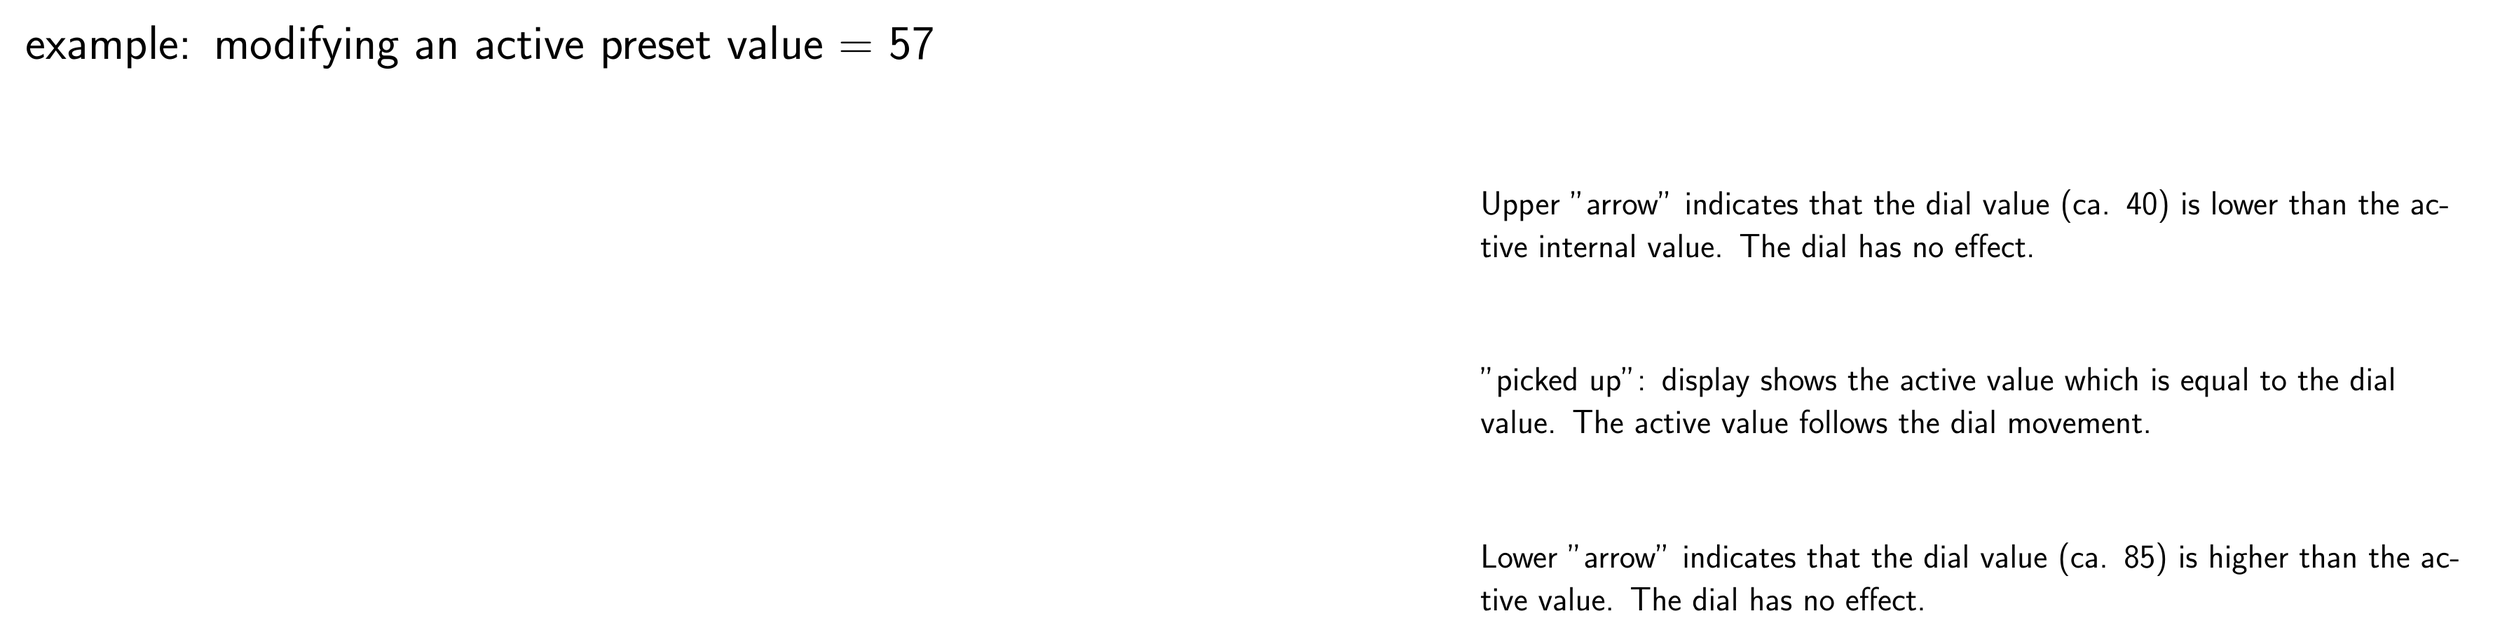
\begin{tikzpicture}[scale=0.8]
  \node[font=\fontsize{24}{22}\selectfont, align=left, outer sep=0.5mm, anchor = west, text width=40cm] at (3cm,20cm) {\presetpanel example: modifying an active preset value = 57};
    \upperbuttons{6.5cm,7.5cm}{PT}{}

    \prophetpot{26cm,8cm}{}{345}
    \prophetdisplay{32cm,8cm}{567}{}{}
    \node[font=\fontsize{18}{22}\selectfont, align=left, anchor = west, text width=18cm] at (36cm,8cm) {Lower "arrow" indicates that the dial value (ca. 85) is higher than the active value. The dial has no effect.};

    \prophetpot{26cm,12cm}{}{65}
    \prophetdisplay{32cm,12cm}{13467}{123}{}
    \node[font=\fontsize{18}{22}\selectfont, align=left, anchor = west, text width=18cm] at (36cm,12cm) {"picked up": display shows the active value which is equal to the dial value. The active value follows the dial movement.};

    \prophetpot{26cm,16cm}{}{125}
    \prophetdisplay{32cm,16cm}{}{237}{}
    \node[font=\fontsize{18}{22}\selectfont, align=left, anchor = west, text width=18cm] at (36cm,16cm) {Upper "arrow" indicates that the dial value (ca. 40) is lower than the active internal value. The dial has no effect.};
    
  \end{tikzpicture}
}

The pick-me-up mechanism avoids discontinuous value changes and it provides a means to dial the current panel into the patch you are hearing. Note, however, that it is important to observe the display and current pick-up status of dials to avoid confusion. If you want a direct application of a dial press \totape to switch back to standard \presetpatch where all control changes are directly applied. The pick-up status of each control is remembered when switching between the two modes.

There is no pick-up mechanism for switches on the panel\footnote{The attempt to do this was made, but surprisingly, the hardware is not reliable enough for this, in particular, the three-way tracking switch.}. The mechanism is also irrelevant for additional patch parameters as there is no conflict between physical controls and internally applied values. Furthermore, the logic applies only to patch parameters. It is not applied to \mastertune, \mastervol, \pitchbender and \modwheel.

Note that the pick-up relies on that your dials can reach the maximum value. If your maximum value as shown on the display is less than 99 you may find that you cannot pick-up patch parameter values close to 99. In this case you should check the DAC gain to see if your instrument falls short of the required 4.9V which correspond to the maximum value. Please consult the service manual on this \cite{p600siservicemanual}. As a work around you can always switch to \presetpatch, change the dial in question and then return to \presetpanel.

\textbf{Default Patch}

Pressing the \preset button (with confirmation) in \shiftmode or \shiftlock loads a default patch (see section \ref{defaultpatch}). After loading the default patch the Prophet-600 is in \presetpatch.


\section{Loading and storing presets}\label{loadstorepatches}

Patches are stored in \storagemode. To enter this mode from \presetmode or \livemode press the \record button, whose LED starts blinking. The Prophet 600 is then waiting for the user to enter the (two-digit) target patch number on the \termnumberpad. Once the second digit is entered, the patch is stored automatically and the LED of the \record button deactivates. 

Loading patches is done by entering \presetpatch and then selecting the patch on the \termnumberpad. Once selected there is a short confirmation on the display.

While the Prophet 600 waits for patch number entry (e.g. \storagemode or \presetpatch) other functions of the \termnumberpad and display (e.g. in \presetpanel or \livemode) are temporarily suppressed. If you find you have accidentally started typing a digit in these modes while expecting to select a patch parameter you can switch / cancel the mode after the first digit, e.g. pressing \totape in \presetpatch or pressing \record again in \storagemode.

For exporting and importing patches via MIDI SysEx see section \ref{patchmgmt}.


\section{Oscillator and mix}\label{osc}

For each of the six voices the Prophet 600 has two voltage controlled oscillators (VCOs) \footnote{The oscillators are Curtis CEM3340 chips}, VCO A and VCO B. Each has a dedicated control field on the panel. The oscillators are identical, offering three waveforms: \textit{sawtooth}, \textit{triangle} and \textit{pulse}. The pulse width of the pulse shape can be adjusted using the corresponding \textbf{Pulse Width} dial. All three shapes can be activated simultaneously. 

\begin{center}
\scalebox{0.4}{
  \begin{tikzpicture}[scale=0.8]
    \oscapanel{0,10cm}
    \oscbpanel{0,0cm}
  \end{tikzpicture}
}
\end{center}


Both oscillators have a \textbf{Frequency} dial which determines the range of the oscillators when played from the keyboard or via MIDI.  The granularity of the Frequency dials can be set to \textit{free}, \textit{semitone} or \textit{octave} (the default) to support the users in the processes. The corresponding parameter is the additional patch parameter \textbf{(88) OSC Pitch Mode} (accessible by pressing 8 twice). An additional \textbf{Fine} dial, available for For VCO B only,  allows for fine tuning of the relative frequency. The man purpose of separate Frequency dials per oscillator as pat of a patch is to be able to detune them against one another. This can be used to create thick and lively patches (when pitch difference is small), to create complex timbres with harmonics (when pitch difference is large, typically octaves) or even create intervals (for example fifths). The frequency setting is also an important aspect of the poly-mod, see section \ref{polymod}. 

VCO A has an additional \textbf{Sync} switch. The hardware of the Prophet 600 offers are hard sync of oscillator A to oscillator B, e.g. VCO A is reset to the cycle start when VCO B completes a cycle. 

Finally, the outputs of both oscillators are mixed into one signal before entering the filter and output stages. The mix panel provides an \textbf{OSC A Volume} dial and an \textbf{OSC B Volume} dial for this purpose. The normalised output of both oscillators is about half way of the respective dial. Beyond this, the amplifiers into the filter can be over-driven. This is a new feature of the upgraded firmware.

Note that in the original Prophet 600 setup these two dials had a different function, oscillator mix and glide, respectively. In the firmware upgrade the glide function has been moved to the \textbf{Additional Patch Parameters}, see section \ref{glide}. 


\section{Volume and global tune}

To the right of the panel there two global parameter dials, the \textbf{Master Tune} and \textbf{Volume} dials. The master tuning has a range or approximately $\pm$semitone. It's pupose is to be able to tune the synth to other instruments without touching the internal, relative frequencies of the oscillators and thereby potentially changing the patch.

\section{Filter}\label{filter}

The mix of the two VCOs is routed through a resonant 24db low pass filter (built on a Curtis CEM3372 filter). The control for the filter consists of a \filtercutoff dial regulating the cut-off frequency, and a \filterres dial for the resonance. The \filterenv dial regulates how strongly the cut-off frequency is modulated by the filter envelope. This dial is bipolar, e.g. it supports positive and negatives values (effectively an inverse envelope setting). The display will show values between -50 and 50 depending on position. This is major enhancement compared to the original Prophet 600 firmware.

\begin{center}
\scalebox{0.4}{
  \begin{tikzpicture}[scale=0.8]
    \addpar{-18cm,9.3cm}{\textbf{Filter Limit} \\ With the miscellaneous setting the cut-off frequency can be limited to 22kHz, see section \ref{limitsett} for details.};
    \draw[line width = 2pt, dashed] (-4cm,9.3cm) -- (1cm,9.3cm);

    \addpar{-18cm,3.5cm}{\textbf{\filenv} \\ This modifies the shape and speed of the envelope, e.g. it influences the attack, decay and release phases, see \ref{envelopes} for details};
    \draw[line width = 2pt, dashed] (-4cm,3.5cm) -- (1cm,3.5cm);

    \filterpanel{0,0}
  \end{tikzpicture}
}
\end{center}

The \keyboardtrack switch has the setting \textit{Off}, \textit{1/2} and \textit{Full}. It lifts the cut-off frequency depending on keyboard note, e.g. the cut-off frequency is higher for higher notes. The effect applies to the cut-off frequency resulting from the fixed \filtercutoff setting plus any envelope and LFO modulation, e.g. it applies to the sum.  


\section{Envelopes and routing}\label{envelopes}

As in the original version the upgraded Prophet 600 offers two ADSR envelopes. The first is the filter envelope, which is associated with and routed to the filter cut-off frequency. Its parameters are located in the filter section of the panel. The second envelope is assignable and the parameters have a dedicated Assignable Envelope section on the panel below the filter section \footnote{In the original Prophet 600 as well as in the uprage up to version 2.1 RC3 the assignable enevelope is in fact a dedicated amplitude envelope. Therefore, in the original and in the upgrade compatible panel overlay the panel section of this envelope is marked "Amplifier". Also with the change from version 2.1 to the version 2.2 the additional patch parameter Amplitude Shape has been consequently renamed Assignable Shape.}.

Both envelopes work identically in that they have a classic ADSR setup with an \textbf{Attack} dial, a \textbf{Decay} dial, a \textbf{Sustain} dial and a \textbf{Release} dial. 

\begin{center}
\scalebox{0.4}{
  \begin{tikzpicture}[scale=0.8]
      \adsrpanel{0,0}
  \end{tikzpicture}
}
\end{center}

Compared to the original, the upgraded Prophet 600 provides not only faster and smoother envelopes but also offers new two different envelope speed regimes, \textit{slow} and \textit{fast}, as well as two different envelope shapes, \textit{linear} and \textit{exponential}.

The shape and the speed can be set independently for the filter and the assignable envelope using two additional patch parameters. The parameter \textbf{(5) Assignable Shape} changes the assignable envelope and the parameter \textbf{(55) Filter Shape} changes the filter envelope. Each of the two parameters can take the following values:

\begin{itemize}
  \setlength\itemsep{0cm}
  \item \textit{slow -linear}
  \item \textit{slow - exponential}
  \item \textit{fast - linear}
  \item \textit{fast - exponential}
\end{itemize}
 
 The envelope shapes are shown below:
 
 \scalebox{0.5}{
  \begin{tikzpicture}[scale=0.8]
    \envelopeexp{0,0}{6}{4}{5}{8}{6}

\end{tikzpicture}
  }

The attack, decay and release times in the low and fast setting are listed in he following table. These values are approximate and nominal only. Especially at fast rates, there is natural lag i the build up of voltages, so that real time developments are smeared out.

\begin{center}
  
  \begin{tabular}{ |c|c|c|} 
   \hline
    A, D \& R dial position & slow shape & fast shape \\
   \hline
  0 & 5 ms & 1 ms \\
   \hline
  1 & 12 ms & 3 ms \\
   \hline
  2 & 30 ms & 8 ms \\
   \hline
  3 & 80 ms & 20 ms \\
   \hline
  4 & 200 ms & 50 ms \\
   \hline
  5 & 500 ms & 125 ms \\
   \hline
  6 & 1,2 s & 300 ms \\
   \hline
  7 & 3 s & 800 ms \\
   \hline
  8 & 8 s & 2 s \\
   \hline
  9 & 20 s & 5 s \\
   \hline
  10 & 50 s & 12 s \\
   \hline

  \end{tabular} 
\end{center}

 
In general the envelopes have three potential targets: filter cut-off frequency, amplitude and poly-mod (for this see section \ref{polymod}). The filter envelope is always routed to the filter cut-off frequency and the modulation strength is controlled by the \textbf{Filter Envelope} dial. For the  amplitude and poly-mod targets different routing options exist as described in detail in the section on poly-mod \ref{polymod}. The additional patch parameter \textbf{(555) Envelope Routing} envelope routing is used to select this. The main benefit from the routing options is to make poly-mod independent from the filter dynamics. The default routing is that the poly-mod is target by the filter envelope and the amplitude is modulated by the assignable envelope.

The modulation strength for the amplitude is fixed in the Prophet 600 (e.g. there is no offset) and positive. The modulation strength for the poly-mod is set by the \textbf{Poly-Mod Envelope} dial as explained in section \ref{polymod}. 


\section{Polyphonic, unison and chord mode, voice assignment priority}\label{poly-unison-voice}

The upgraded Prophet 600 can operated in the following voice modes

\begin{itemize}
  \setlength\itemsep{0cm}
  \item \textit{polyphonic}: This mode is set by setting the \textbf{Unison Switch} on the panel to \textit{off}. In this mode any new note is assigned to one of the 6 voices. 
  \item \textit{unison}: This mode is activated by switching the panel \textbf{Unison} switch from \textit{off} to \textit{on} while not holding any keyboard key pressed. In this mode all 6 voices play the same note. Note that using the additional patch parameter \textbf{(8) Detune} to detune the single oscialltors is used to create thickened sounds in unison mode.
  \item \textit{chord}: This mode is activated by switching the panel \textbf{Unison} switch from \textit{off} to \textit{on} while holding down one or more keys (the "chord"). In this mode the synthesizer transposes that chord over the whole keyboard. Note that independently of how many notes the chord contains (and therefore how many voices would be left in principle), only one chord can be played at a time, similar to unison mode.
\end{itemize} 

The choice of voice mode is a patch parameter e.g. is stored with the patch.

Note that in unison/chord voice modes the foot switch does not hold notes but instead can be used to latch a new patterns of notes / chords on the fly without leaving and reactivating the unison mode. To do so, hold down the chord you want to latch in unison/chord mode and press the footswitch. In order to return to normal unison mode pres the fottswitch with no key held down. 

In polyphonic mode the assignment of voices to new played notes can be customized using the additional patch parameter \textbf{(77) Assigner Priority}.New notes will be assigned to voices according to the following priority rules:

\begin{itemize}
  \setlength\itemsep{0cm}
  \item \textit{last}: New notes always play and if 6 voices already playing then the oldest played notes is "stolen".
  \item \textit{low}: A new played note only plays if it is lower than all 6 voices already playing. In \textit{unison} or \textit{chord} mode, legato is active. This is the preferred setting when bass accompaniment is important and the sudden stop of bass notes would create unwanted disruptions. 
  \item \textit{high}: A new played note only plays if it is higher than the 6 voices already playing. In \textit{unison} or \textit{chord} mode, legato is active. This is the preferred setting for a synthesizer lead situation where the sudden stop of a high note would create unwanted disruptions. 
\end{itemize}

The assigner priority of voice mode is a patch parameter e.g. is stored with the patch.

\textbf{Ideas for solo voices}

The assigner priority can be used effectively in combination with the voice modes to customize solo voices. For example combine the priority \textit{high} (or \textit{low}) with ...
\begin{itemize}
  \item ...\textit{unison} mode for a massive legato solo voice
  \item ...\textit{chord} mode with a one one "chord" (hold down C3) to achieve a more delicate legato mono solo voice
  \item ...\textit{chord} mode with octaves (hold down C3 plus C4 plus more if desired) for a more assertive mono solo voice   
\end{itemize}


\section{LFO}\label{lfo}

Like the original model, the upgraded Prophet-600 offers a single main LFO\footnote{There is also a vibrato, see section \ref{vib}}. However, the functionality is substantially enhanced. The frequency range of the LFO is wider, from 1/20 to 60 Hz. There are additional waveforms (a total of 6). The upgraded Prophet-600 offers more modulation target options and, finally, the user has the option to either control the LFO amount using the modulation wheel or to set a modulation delay for the LFO. As a result the controls on the LFO sub-panel shown below are affected by 5 menu parameters. Still, the most important LFO controls can be changed hands-on using the dedicated LFO controls. 


\begin{center}
\scalebox{0.4}{
  \begin{tikzpicture}[scale=0.8]

    \addpar{-18cm,6cm}{\lfoshape \\ You can select 3 pairs of different shapes to be assigned to the \shapeswitch};
    \draw[line width = 2pt, dashed] (-5cm,7.5cm) -- (5cm,7.5cm);

    \addpar{-18cm,0.5cm}{\lfosync \\ This parameter activates LFO synchronisation to internal or external clock on selectable time measures (only active when arp and/or seq are playing)};
    \draw[line width = 2pt, dashed] (-5cm,3.5cm) -- (-0.5cm,3.5cm);

    \addpar{-12cm,11.5cm}{\modwheeltarget \\ The modulation wheel can be set to control the LFO amount};
    \draw[line width = 2pt, dashed] (2cm,12.5cm) -- (10cm,6.5cm);

   \lfosubpanel{-2cm,0}

    \addpar{24cm,11.5cm}{\moddelay \\ The modulation delay applies to the LFO when the modulation wheel controls the vibrato};
    \draw[line width = 2pt, dashed] (23cm,12.5cm) -- (14cm,6.5cm);

    \addpar{28cm,2.5cm}{\lfotarget \\ Different target options include modulating only oscillator A or B and amplitude modulation};
    \draw[line width = 2pt, dashed] (27cm,4.5cm) -- (24.5cm,4.5cm);


  \end{tikzpicture}
}
\end{center}

\textbf{LFO speed}

The LFO speed / frequency is set in the panel using the \lfofreq dial\footnote{Up to the upgrade version 2.1 RC3 a menu parameter was available to chose between slow and fast frequency ranges for the LFO. In the new version the range selection using the \lfofreq control has been made exponential and the control range covers the entire frequency range. The range has also been extended further compared to 2.0 and 2.1 RC3 both on the low end and on the fast end.} 

\textbf{LFO modulation amount and targets}

There are four modulation targets which can be active simultaneously. Three targets are activated using the switches \lfovco (modulation of oscillator pitch), \lfopwm (modulation of pulse width) and \lfofil (modulation of the filter cut-off frequency) in the LFO sub-panel. The modulation amount is set using the \lfoamt control\footnote{The action of the \lfoamt dial has been made exponential and therefore with a slower onset in the lower value range. In particular when pitch modulation is active this provides a longer travel for commonly useful modulation amounts, typically up to 2-3 on the control scale.} and this amount applies to all activated modulation targets at fixed relative strength. The pitch modulation is harmonic and the maximum \lfoamt corresponds to 30 semitones.  

In the upgraded Prophet-600 you can customize the LFO target. The additional patch parameter \lfotarget
offer the settings: 

\begin{itemize}
  \item \textit{A \& B}: Both oscillators are modulated, this is the standard of the original Prophet-600 
  \item \textit{A}: Only VCO A is modulated
  \item \textit{B}: Only VCO B is modulated
  \item \textit{VCA}: Amplitude modulation, and both oscillators are selected for all targets
\end{itemize}

The choices for oscillators A and B affect the targets \textit{VCO} and \textit{PWM} but obviously not \textit{Filter} as there is only one filter per voice. When the target \textit{VCA} is selected, both oscillators are targets for \textit{VCO} and \textit{PWM} modulation (if the respective switches are on). 

\textbf{LFO shapes}

The upgraded Prophet-600 supports not only the waveform \textit{Pulse} and \textit{Triangle} of the original model but four additional shapes, \textit{Sin}, \textit{Sawtooth}, \textit{Random} and \textit{Noise}. On the sub-panel there is one simple up/down \shapeswitch switch. To accommodate 6 waveforms an additional patch parameter \lfoshape is used. Selecting the desired waveform therefore requires selecting the respective shape pair and then using the \shapeswitch switch to toggle between the two shapes. 

\begin{center}
\begin{tabular}{ |l|l|l|} 
 \hline
  \lfoshape set to: & \shapeswitch \textit{up} & \shapeswitch \textit{down} \\
 \hline
 \textit{tri-pulse} & LFO shape is triangle & LFO shape is square\\
 \hline
 \textit{sin-random} & LFO shape is sin & LFO shape is random \\
 \hline
 \textit{saw-noise} & LFO shape is sawtooth & LFO shape is noise \\
 \hline
\end{tabular}
\end{center}

\textbf{LFO delay and modulation of LFO}

The strength LFO effect itself can be modulated by either the modulation wheel or a delay function. Using the menu parameter \modwheeltarget your can choose \textit{vibrato} or \textit{LFO}. When set to \textit{LFO} the modulation wheel controls the LFO amount. The LFO starts at initial amount as set by \lfoamt on the sub-panel and turning the modulation wheel up adds LFO strength. The wheel action itself is set using the menu parameter \modwheelrange. If the modulation wheel target is set to \textit{vibrato} then, automatically, the modulation delay is applied to the LFO, i.e. the LFO onset is delayed by the amount set by the menu parameter \moddelay. For details on modulation wheel related parameters see section \ref{modwheel}.

\textbf{LFO re-triggering}

As a new feature in version \version, the re-triggering behavior of the LFO can be customized. The default is a free running LFO, but you can also set the LFO to re-trigger with new played keys (i.e. when no key is held and a new key is played) or to re-trigger depending on (external or internal) clock. The latter effectively syncs the LFO to the arpeggiator and/or sequencer. The menu parameter \lfosync provides the choices \textit{off} (free running LFO), \textit{key} and \textit{1, 2, 3, 4, 5, 6, 8} to have the LFO reset after 1, 2, 3, 4, 5, 6 or 8 beats or the arpeggiator and/or sequencer. The LFO clock sync is only active if arpeggiator and/or sequencer is running. For details on clock settings see \ref{sync}.


\section{Poly-Mod}\label{polymod}

The functions associated with the poly-mod section are very powerful. They provide the means for non-linear modulation: cross-modulattion of the two voice oscillators and also to modulation the filter cut-off frequency by VCO B. 

The familiar and common synthesizer feature is that the oscillator (frequency,filter  cut-off frequency, pulse width, etc.) is modulated by a \textit{low frequency oscillator (LFO)}. An LFO does not operate in the audible frequency range (it is "low frequency") and it has a fixe frequency, e.g. independent from the note played. Poly-mod is different in that the modulation itself is in the audible range and the resulting non-linearity changes the frequency spectrum drastically. The resulting effect is compareable to FM synthesis known from digital synthesizers, although in the Prophet 600 it is more raw and fully analog. Like the oscillator sync function, cross-modulation is hardware implemented.

The poly-mod control can be found in the poly-mod sub-panel. 

\begin{center}
\scalebox{0.4}{
  
\begin{tikzpicture}[scale=0.8]

    \addpar{-18cm,3.5cm}{\envrouting \\ The routing options determine whether poly-mod is driven by the filter or the 2nd envelope};
    \draw[line width = 2pt, dashed] (-4cm,3.5cm) -- (1cm,3.5cm);


   \polymodesubpanel{0,0}
  \end{tikzpicture}
}
\end{center}

There are two modulation sources, \polyenv and \oscamt and two destinations, oscillator a pitch and filter cut-off frequency, which are activated using the respective panel switches \plyfreqa and \plyfilter. The \oscamt control determines how strongly the oscillator B modulates poly-mod targets (destinations). It is instructive to consider the effect of oscillator B modulation on the two targets first and then explore the effect of envelope modulation.

\textbf{Cross-modulation}

\begin{itemize}
  \item When setting the \plyfreqa switch to \textit{on}, oscillator B modulates the frequency of oscillator A, e.g. frequency modulation (FM). Depending on the modulation strength the result is a wide and rich frequency spectrum which contains among others the sum and difference of multiples of the two oscillators frequencies . The spetrum strongly depends on the frequency difference and may be totally non-harmonic but also harmonic for carefully adjusted frequency settings. Typical spectra are often described as bell sounding. Note that in contrast to FM synthesizers which use highly accurate sin waves, the oscillator output of the Prophet does not have the same basic accuracy and the available waveforms already contain higher harmonics. Therefore the FM result in the Prophet 600 is typically more drastic and dirtier and requires classic subtractive methods for shaping the sound, e.g. the application of the low pass filter. 
  \item When setting the \plyfilter switch to \textit{on}, oscillator B modulates the filter cut-off frequency of the VCF. Like frequency modulation this is a non-linear modulation. This effect can also produce a wide frequency spectrum which may or may not be harmonic, depending on the relative frequency of oscillators A and B. The effect is more pronunced at low filter cutt-off frequencies. The resonance also has a strong effect.  
\end{itemize}

Note that poly-mod is very tuning sensitive and that it maybe necessary to retune the synth more often when using extreme poly-mod settings.

\textbf{Envelope modulation}

The second modulation source in the poly-mod envelope whose strength set by the \polyenv dial. This activates a pitch modulation of oscillator A using an envelope when the Frequency switch is \textit{on}. The \polyenv control is bipolar, that is it provides negative (inverse modulation) and positive values. Note that the poly-mod envelope only affects the frequency of oscillator A. The filter cut-off frequency is already modulated by the filter envelope. 

The pitch modulation by envelope is not a cross-modulation function. However, the association with poly-mod is useful because of the drastic effect of frequency (differences) on the sound spectrum. By time modulating the pitch, the sound can be made to sweep through different spectra, ranging from apocalyptic noise through bell sounds to delicate transients. The way humans perceive natural sounds is strongly influenced by the frequency characteristics of the transients (typically short lived high frequency components) in the attack and decay phases of the sound. This is best modelled using an envelope making it a versatile tool for advanced sound design. 

IN order to further expand the sound design posisbilities, the latest firmware upgrade offers envelope routing   option. The menu parameter \envrouting determines if the filter envelope or the assignable envelope is used in poly-mod\footnote{Up to version 2.1 RC3 the filter envelope was "hard wired" to poly-mod.}. The following figure provides an overview of the routing options. Having different envelopes modulating the filter and the poly-mod opens up new possibilites in the sound and spectrum dynamics. 

\begin{itemize}
  \setlength\itemsep{0cm}
  \item \textit{standard}: In this "standard" routing the amplitude is modulated by the 2nd envelope and the poly-mod is modulated by the filter envelope. This is the setup of the original Prophet 600. 
  \item \textit{poly-amplitude}: In this routing both the amplitude and the poly-mod are modulated by the 2nd envelope. 
  \item \textit{poly}: In this routing the amplitude is modulated by the filter envelope and the poly-mod is modulated exclusively by the 2nd envelope. Therefore the poly-mod time modulation is completely free, at the expense of having filter modulation and amplitude tied together.
  \item \textit{gate}: In this routing the amplitude is not modulated at all, but behaves like a gate (similar to electronic organs). The poly-mod is modulated exclusively by the assignable envelope. Therefore the poly-mod modulation is completely free at the expense of have a less dynamic sound evolution.
\end{itemize}  

\scalebox{0.4}{
  \begin{tikzpicture}[scale=0.8]
   \envroute{0,0}
  \end{tikzpicture}
}

\textbf{Oscillator sync and poly-mod}

As explained in section \ref{osc}, oscillator A can be sync'ed to oscillator B using the \oscsync switch in the sub-panel for oscillator B. This can also be view as a variant of cross-modulation. The sync function can even be combined with frequency modulation as decribed above. 

Combining oscillator sync with poly-mod pitch modulation by envelope can be used to produce interesting short transients or slow sound evolutions. For example, when oscillator A is a pulse wave, then sync'ing this wave to oscillator B and time modulating the pitch of oscillator A has the effect of pulse width modulation by envelope. It creates a change in timbre which can be short to simulate plucking an brassy attacks or long to produce a sweep of the sound spectrum.

\textbf{Starting points for patch design with poly-mod and sync}

Using poly-mod in combination with oscillator sync, different modulations strengths for different oscillator pitches with different filter and modulation shapes is a ver wide field of experimentation. Here are some ideas as potential starting points

\begin{itemize}
  \item Set the envelope routing to \textit{standard}, tune both oscillators to the same frequency, in the poly-mod scetion turn source VCO B to zero and deactivate the filter modulation. Then set VCO A to sync and experiment with the poly-mod envelope source amount. This produces a sync whic, for high envelope amounts, can be tuned to a quite harsh synth solo sound.
  \item ... (to be done)
\end{itemize} 


\section{Arpeggiator}\label{arp}

The upgraded Prophet-600 supports the three arpeggiator patterns \textit{up/down}\footnote{The pattern is different in firmware versions 2.0 and 2.1 RC3: the lowest and highest note in the up/down pattern were played twice (e.g. "1234432112...") while now they are only played once (e.g. "12343212...").}, \textit{assign} and \textit{random}\footnote{In firmware  versions 2.0 and 2.1 RC3 the random pattern was slightly different. Formerly, a single note could be randomly repeated two or more times while now a note is never repeated (unless there is only one note to play).}  which are activated using the arpeggiator buttons as described in the following.

\scalebox{0.4}{
  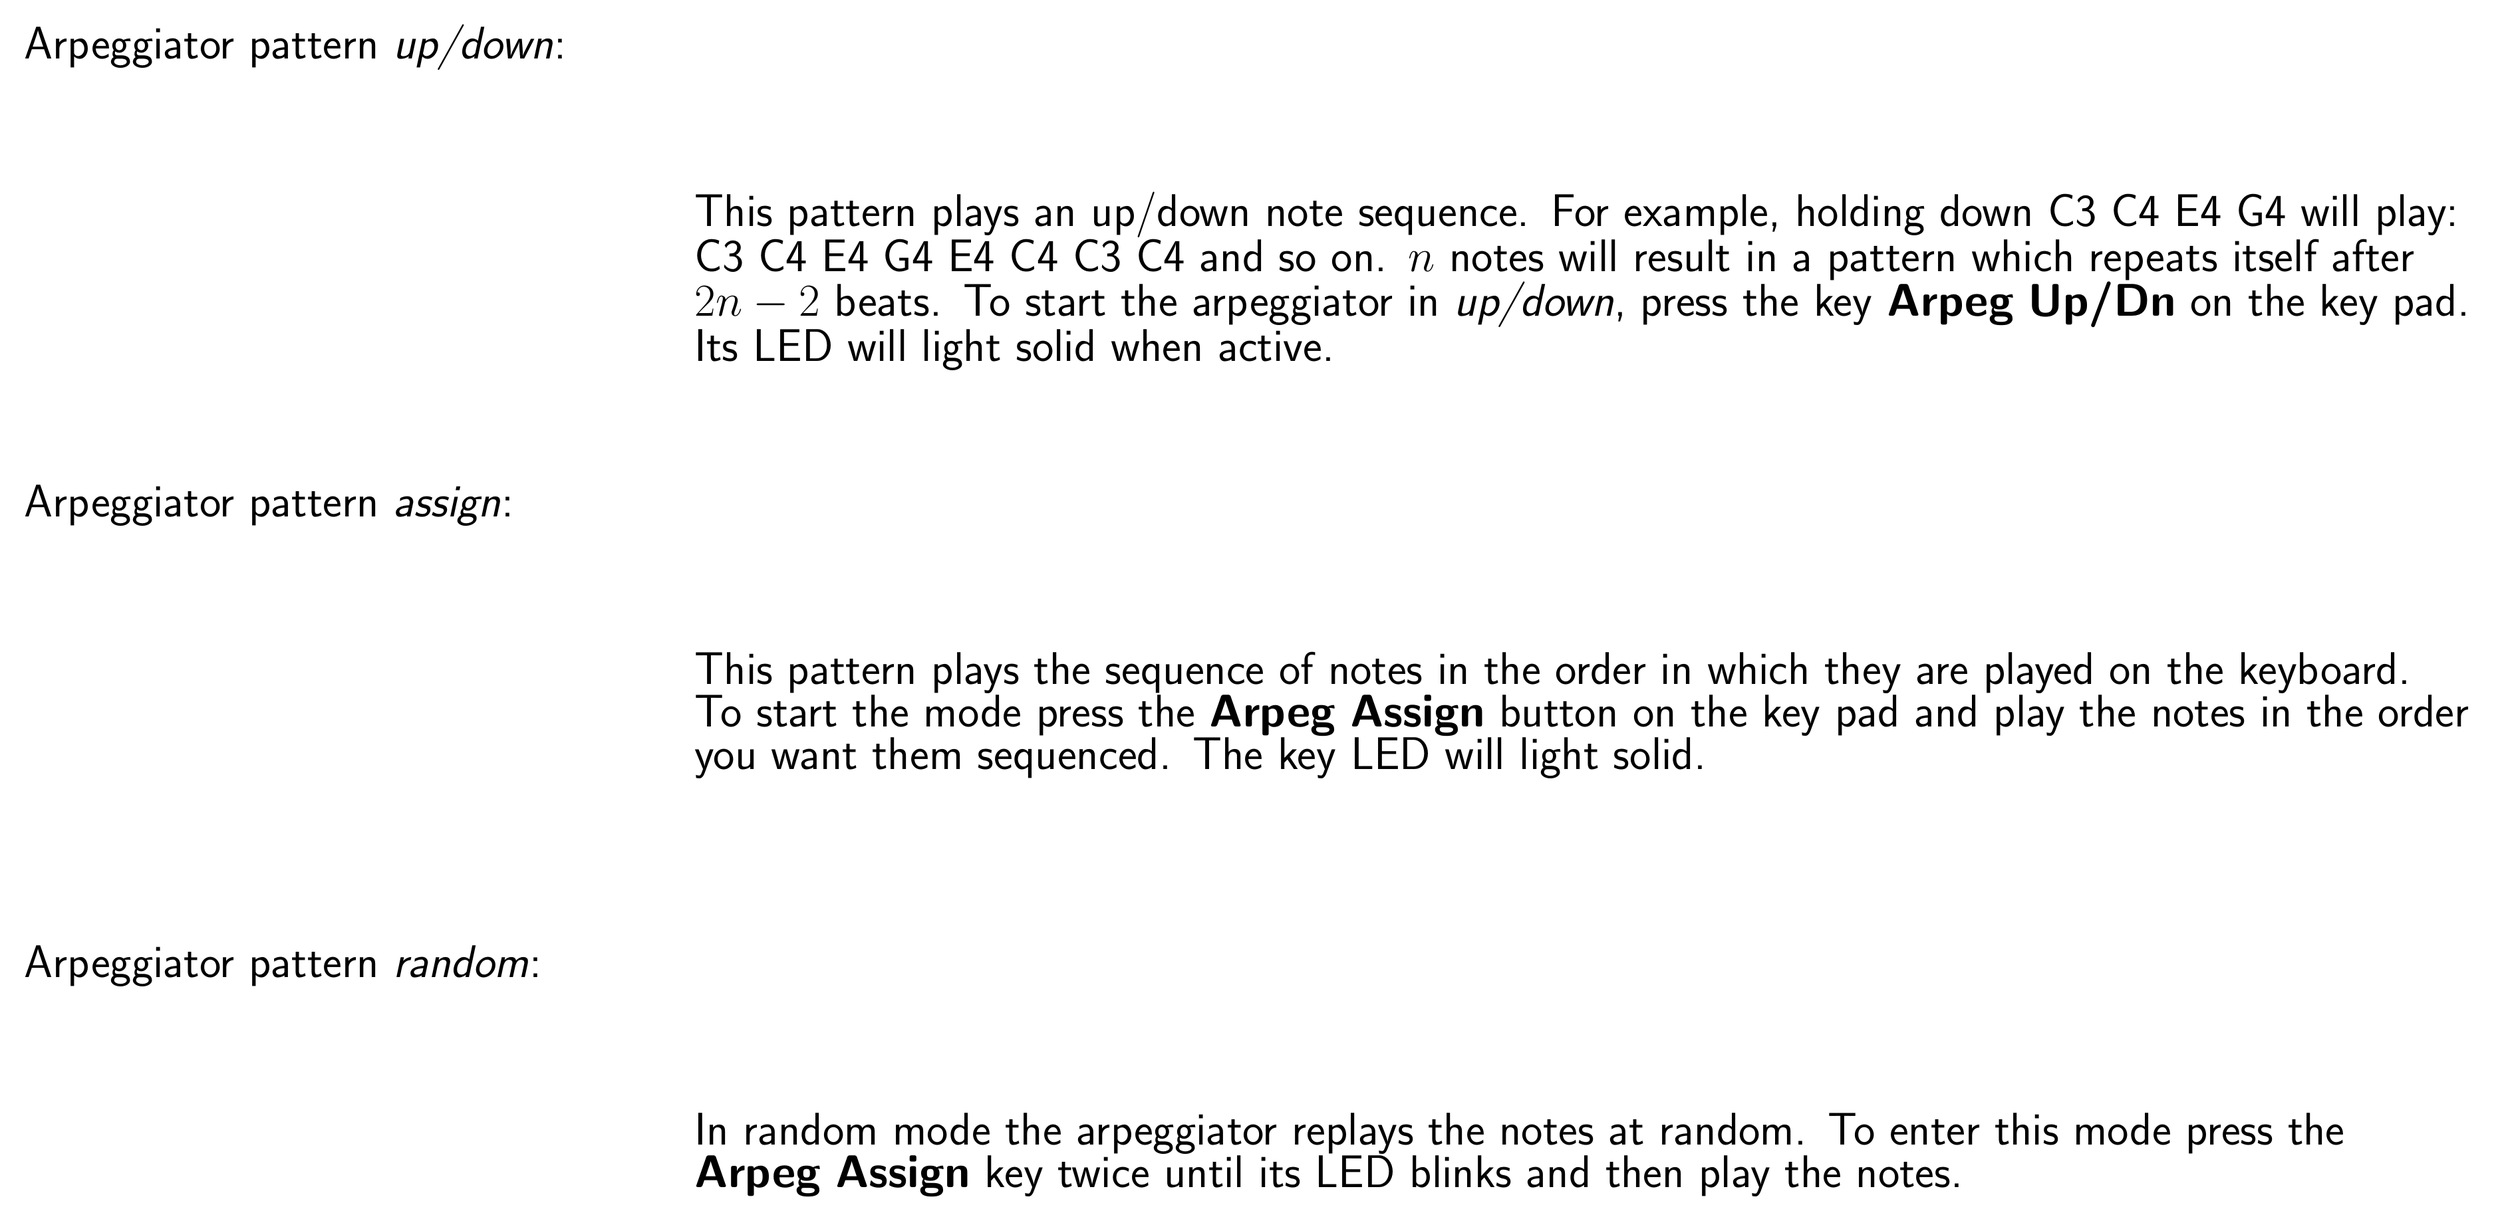
\begin{tikzpicture}[scale=0.8]
  \node[font=\fontsize{26}{22}\selectfont, align=left, outer sep=0.5mm, anchor = north west, text width=30cm] at (0cm,31cm) {Arpeggiator pattern \textit{up/down}:};
  \node[font=\fontsize{26}{22}\selectfont, align=left, outer sep=0.5mm, anchor = north west, text width=34cm] at (16cm,27cm) {This pattern plays an up/down note sequence. For example, holding down C3 C4 E4 G4 will play: C3 C4 E4 G4 E4 C4 C3 C4 and so on. $n$ notes will result in a pattern which repeats itself after $2n-2$ beats. To start the arpeggiator in \textit{up/down}, press the key \textbf{Arpeg Up/Dn} on the key pad. Its LED will light solid when active.};
    \arpsqbuttons{1cm, 22cm}{U}{}
    
  \node[font=\fontsize{26}{22}\selectfont, align=left, outer sep=0.5mm, anchor = north west, text width=30cm] at (0cm,20cm) {Arpeggiator pattern \textit{assign}:};
  \node[font=\fontsize{26}{22}\selectfont, align=left, outer sep=0.5mm, anchor = north west, text width=34cm] at (16cm,16cm) {This pattern plays the sequence of notes in the order in which they are played on the keyboard. To start the mode press the \textbf{Arpeg Assign} button on the key pad and play the notes in the order you want them sequenced. The key LED will light solid.};
    \arpsqbuttons{1cm, 11cm}{A}{}

    
  \node[font=\fontsize{26}{22}\selectfont, align=left, outer sep=0.5mm, anchor = north west, text width=30cm] at (0cm,9cm) {Arpeggiator pattern \textit{random}:};
  \node[font=\fontsize{26}{22}\selectfont, align=left, outer sep=0.5mm, anchor = north west, text width=34cm] at (16cm,5cm) {In random  mode the arpeggiator replays the notes at random. To enter this mode press the \textbf{Arpeg Assign} key twice until its LED blinks and then play the notes.};
    \arpsqbuttons{1cm, 0cm}{A}{A}
  \end{tikzpicture}
}

It is possible to sync the LFO to the arpeggiator using the additional patch parameter \clocksync, see section \ref{sync}.

\textbf{Latch mode}

With all arpeggiator modes, press the \record button on the key pad to enter the arpeggiator latch mode in which played notes are held, i.e. are sustained after the keys are released. The LED of the \record button will light solid. Playing additional notes in this mode will add them as additional notes to the existing sequence, up to a maximum of 128 notes. To clear the notes from the sequence, press the \record button to switch the latch mode off. The LED of the Record button will go off.

The foot switch has the same function as pressing \record while the arpeggiator is running. It toggles the arpeggiator latch mode as indicated by the \record LED. 

\textbf{Transposition}

The arpeggiator pattern can be transposed on the fly. To do so use the keyboard in \shiftmode or \shiftlock, see section \ref{transposition}.

\textbf{Controlling the arpeggiator using MIDI}

It is possible to input notes into the arpeggiator via MIDI. The MIDI behaviour in this context depends on the MIDI mode (\textit{local on} or \textit{local off}, see section \ref{midiintegration}) in the following way when the arpeggiator is running:

\begin{itemize}
  \item \textit{local on}: Keys played on the keyboard are entered into the arpeggiator. Transposition works normally. MIDI notes sent to the Prophet-600 play normally. This means that they are not sent to the arpeggiator but play on top of the running arpeggiator.
  \item \textit{local off}: Keys played on the keyboard are not entered into the arpeggiator but are sent out as MIDI in the normal way. Transposition of the arpeggiator works from the keyboard and from external MIDI. MIDI notes sent to the Prophet-600 are input into the arpeggiator. MIDI cannot play normally on top of the arpeggiator. 
\end{itemize}

\textbf{Troubleshooting}

If the arpeggiator is activated and keys are held down or have been latched and still no sound plays, then it is worth checking the following potential reasons: Is the sync set to \textit{internal} and is the \clock greater than zero? If the sync is not \textit{internal} does the instrument receive a clock via MIDI on the correct channel or via tape in? If the instrument in \textit{local on} mode (see section \ref{midiintegration})?


\section{Sequencer}\label{seq}

The live sequencer of the original Prophet 600 has been replaced by a step sequencer which supports polyphony. Two sequences can be stored per patch and can play simultaneously. Sequence 1 is started by pressing the key \textbf{SEQ 1}, sequence 2 is started by pushing the button \textbf{SEQ 2}. The LED of the running sequencer is on. Live sound control via panel controls, menu parameters and MIDI CC as well as playing via keyboard and/or MIDI is fully supported while the sequencer is running. To stop either sequence, press the respective sequencer button again. The LED of the stopped sequencer is off. 

It is possible to sync the LFO to the arpeggiator using the additional patch parameter \textbf{(111) LFO Sync}, see section \ref{lfo}.

By default the sequences are empty, so even with the started sequencer no sound will play. If either sequence is activated and no sound plays, then it is worth checking the following potential reasons: Has a note been added? Is the sync set to \textit{internal} and is the speed greater than zero? If the sync is not \textit{internal} does the instrument receive a clock, e.g. via MIDI on the correct channel or via tape in?

\textbf{Tempo}

The tempo of the sequencer is set by the \textbf{Speed} dial. To activate the tempo function the \textbf{(0) Seq/Arp Speed} parameter must be selected. Note that while in sequencer record mode (see below) the button \textbf{To Tape} has to be activated (its LED is lit solid) to select additional patch parameters via the number pad and also to switch on the speed dial. The  sequencer can be synced to external sources. The miscellaneous setting \textbf{Clock Sync} (setting 8) provides the choices \textit{internal}, \textit{MIDI} or \textit{Tape In} (see also section \ref{sync}).

\textbf{Creating / editing a sequence}

The following is an example work flow for adding notes, rests and ties to a sequence and covers all editing functions needed. 

\begin{enumerate}
  \item Press the \textbf{Record} button. Its LED starts flashing.
  \item Press the sequencer button of the sequence you would like to edit (SEQ 1 or SEQ 2). The LED of the respective sequencer button starts flashing, and the Record button light becomes solid. The sequence is in record mode an awaits notes, rest to be added to the sequence.Note: The sequencer is running in this mode, so as soon as the first note is entered this note is repeatedly replayed at the current sequencer/arpeggiator tempo. If notes have previously been added to the sequence, this sequence is played and any new notes are added. 
  \item Adjuts he tempo as described above. Note that you can set the Speed dial to control the tempot before starting the record mode. The parameter selection is preserved. Be careful when selecting the parameter in record mode. It requires pushing and holding  the \textbf{To Tape} button. Otherwise pushing the "0" button has a different, sequencer specific function: it resets the sequence.  
  \item Play the notes to be added to the sequence. The display screen shows which step is currently being added, e.g. it is the current length of the recorded sequence including rests and ties.
  \item Pressing "0" on the keypad resets the sequence and deletes any notes. Note: there is no confirmation step. 
  \item In sequencer record mode the “2” key on the number pad is used for both rests and ties. It adds a rest when no key is pressed, and a tie when a key is pressed.
  \item Added notes (or chords), ties and rests can be successively deleted/undone using the "1" key on the number pad. 
  \item In order to complete the sequence editing and to leave the record mode, press the respective sequencer button (\textbf{SEQ 1} or \textbf{SEQ 2}). The sequencer button LED becomes solid, and the \textbf{RECORD} button LED does off. The sequence is saved. 
\end{enumerate}

\textbf{Transposing a  sequence}

To transpose a sequence, hold the \textbf{From Tape} button and then press the key on the keyboard to which the sequence should be transposed. The C3 key is zero or standard tuning, and will not transpose. Playing C sharp 3 will transpose the sequence up a half step, playing D3 will transpose the sequence up a whole step, etc.


\section{Vibrato}\label{vib}

The upgraded Prophet-600 features a dedicated vibrato. Its parameters are available in the additional patch parameter menu as follows.

\begin{itemize}
  \item The \vibspeed sets the vibrato frequency in a range of approximately 1/20 to 60 Hz
  \item The \vibamt sets the vibrato strength
  \item The \vibtgt sets the vibrato target. The options are \textit{VCO} (modulating the pitch of oscillators A  and B), \textit{VCA} (modulating the amplitude) as well as \textit{VCO A} and \textit{VCO B}(modulating only the pitch of one oscillator A  or  B, respectively)
\end{itemize}

The vibrato shape is a triangle wave. The vibrato effect can be controlled by either the modulation wheel or a modulation delay function. The additional patch parameter \modwheeltarget can be set to \textit{vibrato} or \textit{LFO}. When set to \textit{vibrato}, pushing the \modwheel up adds vibrato strength. The strength of the \modwheel is controlled by the additional patch parameter \modwheelrange. If you set the \modwheel target to \textit{LFO}, on the other hand, the modulation delay is automatically applied to the vibrato, i.e. the vibrato onset is delayed by the amount set by the additional patch parameter \moddelay. For setting the parameters of the modulation wheel see section \ref{modwheel}. For complementary functions for LFO see section \ref{lfo}.


\section{Pitch bender}\label{pitchbend}

The Prophet-600 comes with a (pitch) \textbf{Bender} (without automatic return to the middle position). With the upgrade it is possible to customize the range/action and the target of the bender as part of the patch configuration (see below). 

Note: External MIDI pitch bend is \underline{added} to the internal pitch bend\footnote{This is the behaviour of the original firmware. Since the bender does not return to zero a bend override by external MIDI leads to unwanted discontinuous pitch changes when the bender of the Prophet-600 is touched. The addition of both bends is therefore more consistent.}. Full internal and external (MIDI) bend covers twice the range set by the bender range. As a consequence, the external MIDI bend value cannot be reset/overridden using the built in bender, but the external value is reverted to zero during the bender calibration process (see below).

\begin{itemize}
  \item The bender can target the oscillator pitch, the filter cut-off frequency or the amplitude. This is set using the additional patch parameter \bentarget which provides the options \textit{off}, \textit{AB} (bend of the pitch of both oscillators), \textit{VCF} (modulating the cut-off frequency), \textit{volume} (modulating the amplitude) and \textit{b} (bending the pitch of oscillator B only).
  \item The range of the bender can be configured using the additional patch parameter \bendrange. It offers the choices \textit{2nd} (bend a full tone), \textit{3rd} (bend 4 semi-tones), \textit{5th} (bend 7 semi-tones) and \textit{octave} (bending an entire octave).
\end{itemize}

The upgraded Prophet-600 also offers the option to calibrate the bender middle position using one of the miscellaneous settings/function (see section \ref{settingsref}). This function is useful to remove jittery behaviour of the bender around the middle position. In order to calibrate the bender follow the steps below.

\begin{enumerate}
  \item Move the bender to the middle position.  
  \item Activate bender calibration by pressing \numberbut{3} in \shiftmode or \shiftlock (the display will show that the bender calibration mode is active). Pressing \numberbut{3} again applies and confirms the calibration and exits the calibration mode.
\end{enumerate}

As mentioned above, the current active external (MIDI) bend value is set to zero during the calibration process. To be precise, it is set to zero with the first press of \numberbut{3} in \shiftmode or \shiftlock.


\section{Modulation wheel and modulation delay}\label{modwheel}

The upgraded Prophet-600 has two methods for controlling the modulation effect of the LFO and the vibrato and these properties are  stored with the patch. The first one is the \modwheel. The target of the modulation wheel can be set using the menu patch parameter \modwheeltarget which provides the options \textit{LFO} and \textit{vibrato}. 

The second method is a modulation delay which delays the onset of the modulation effect. The delay is always applied to the modulation source which is \underline{not controlled} by the \modwheel. So when the modulation wheel target is set to \textit{LFO} the delay applies to the vibrato and when it is set to \textit{vibrato} the delay is applied to the LFO.

The target setting as well as the modulation wheel strength and the delay time are set as follows. 
\begin{itemize}
  \item \modwheeltarget provides choices \textit{LFO} and \textit{vibrato}
  \item \moddelay is a continuous menu parameter (range 0...99) which controls the delay time
  \item \modwheelrange offers 4 options: \textit{touch}, \textit{soft} (this is the default), \textit{high} and \textit{full}
\end{itemize} 

The parameter \modwheelrange affects the \modwheel action for all variations except \textit{VCA}. If the target is \textit{vibrato} and the vibrato target is \textit{VCA} the wheel action is always effectively \textit{full}. The reason is that amplitude modulation is a weak effect and there is no practical value in making the \modwheel softer in this case.

Note: the \modwheel action has been modified in all settings compared to version 2.0 and 2.1 RC3. It is now exponential to provide a smooth onset for better playability.


\section{Glide}\label{glide}

In the original Prophet 600 the glide setting (the glide time) had a dedicated dial. In the upgraded Prophet 600 the dial has been re-designated to control the amplitude of OSC B. As a consequence the glide time has been moved to the additional patch parameter \textbf{(7) Glide}. 

\section{Detune}\label{detune}

The upgraded Prophet 600 provides a method to detune the 6 voices against one another. This effect can be used in particular to make unison sound broader and more lively. The additional patch parameter is \textbf{(77) Detune}

\chapter{Synthesizer setup and maintenance}

\section{Tuning}\label{tuning}

The Prophet 600 is a VCO synthesizer, e.g. the frequency of the oscillators A and B are set by apllying a voltage to the control pin of the microchip. The relationship between absolute voltage and resulting frequency is not precise. It depends on many factors, such as smallest differences in the manufacturing process of the chip itself and the surrounding circuit components and operating temparture (the temparture of the components also changes during operation). Therefore the synthesizer need to be tuned regularly. Typically, tuning is best after the instrument (or rather: the chips and components) has been given time to warm up to a stable operating temperature, which could be 10-30 minutes into operation. It may be necessary to retune the synth during operation. The user should trust her or his ear on this.

The automated tuning procedure applies 12 note equal tempered tuning. For other tunings each of the 12 notes can be tuned manually. The per note tuning is stored as part of the patch (in contrast to the overall tuning, which is stored as part of the settings and applies to all presets) and it is retained after full tuning. To enter the per note tuning hold down From Tape and press Tune. The Tune button flashes. In this mode the last played note is tuned using the mod wheel. From the middle position the tune range is $\pm$1 semitone from equal tempered. To leave the per note tuning mode press Tune again.

\section{MIDI integration}\label{midiintegration}

For supporting the integration of the Prophet 600 in a studio or live environment using MIDI, several MIDI functions are supported.

\begin{itemize}
  \item Note send and receive
  \item Control of many parameters using MIDI CC
  \item Local on and local off modes
  \item SysEx support for patch management (for this see section \ref{patchmgmt})
\end{itemize}

The MIDI send and receive channels can be set using dedicated miscellaneous settings as follows. In \shiftmode or \shiftlock:

\begin{enumerate}
  \setlength\itemsep{0cm}
  \item \numberbut{1} cycles through the MIDI receive channels, from \textit{OMNI} through channels \textit{Ch1} to \textit{Ch16}
  \item \numberbut{2}  cycles through the MIDI send channels, from \textit{Ch1} to \textit{Ch16}
\end{enumerate}

\textbf{Notes, performance and MIDI CC}

The Prophet 600 sends the following MIDI signals. 

\begin{enumerate}
  \setlength\itemsep{0cm}
  \item Key on, key off in all modes
  \item Pitch bender
  \item Hold pedal (in polyphonic mode, not in unison/chord mode or running arpeggiator or sequencer)
  \item Modulation wheel (technically a MIDI CC event)
  \item Program change (technically a MIDI CC event)
\end{enumerate}

All of the events can also be received and executed with the following exceptions/modifications.

\begin{enumerate}
  \setlength\itemsep{0cm}
  \item Unlike the internal key on/off events, in arpeggiator mode incoming MIDI key on/off are not entered into arpeggiator but play normally 
  \item Unlike the internal key on/off events, in \shiftmode or \shiftlock incoming MIDI notes do no cause transpositions (but are ignored) 
  \item External MIDI pitch bend is added to the pitch bend from the on-board bender 
  \item MIDI Hold Pedal events are also applied in unison/chord mode or running arpeggiator or sequencer where it has the effect of latching notes/chords
  \item MIDI program change messages are only applied in \presetmode and are ignored otherwise  
\end{enumerate}

The instrument does not send MIDI CC (apart from modulation wheel and program change). However, the Prophet 600 supports a comprehensive list of general and specific MIDI CC events. For reference see section \ref{midiimplementation}. Incoming MIDI CC events are only applied in \presetmode.

\textbf{Local off mode}

The Prophet 600 supports a \textit{local off} mode which is toggled using the setting at \numberbut{0}. In \textit{local off} mode various internal events (such as notes) are not executed in the Prophet 600 directly but they are still sent as MIDI events. The typical setup would be to connect to a MIDI recorder and feed the recorded MIDI messages back to the instrument for replay. The \textit{local off} mode ensures that there is no doubling of events.

Note that in \textit{local on} mode external MIDI does not play into the arpeggiator but plays over the arpeggiator while the local keyboard plays into the arpeggiator. Since the arpeggiator and the playing the external MIDI notes share the 6 voices this can lead to interference of the two, such as missed arpeggiator notes, depending on what play using MIDI. 

\textbf{Overview of MIDI integration}

\begin{table}[H]
  \begin{tabular}{lcccccc}
     &
      \multicolumn{3}{c}{\textit{local on}} &
      \multicolumn{3}{c}{\textit{local off}} \\   \cline{2-7} 
    & Apply local & Send MIDI & Apply MIDI & Apply local & Send MIDI & Apply MIDI \\
    \hline
      \vline Keys on/off playing	& Yes & Yes	& Yes & No & Yes & Yes \\
      Keys into arpeggiator	& Yes & Yes	& No\footnote{MIDI notes will play normally / freely on top of the running arpeggiator. note that voice sharing between arpeggiator and playing MIDI notes can lead to unwanted interference such as missed arpeggiator notes etc.} & No & Yes & Yes \\
      Keys into sequencer	& Yes & Yes	& Yes & No & Yes & Yes \\
      Modulation Wheel	& Yes & Yes	& Yes & No & Yes & Yes \\
      Pitch Bend	& Yes & Yes	& Added & No & Yes & Yes \\
      Program Change	& Yes & Yes	& in preset mode & Yes & Yes & in preset mode \\
      Pedal Hold (Latch)	& Yes & No & No & Yes & No & No \\
      Pedal Hold (Sustain)	& Yes & Yes & Yes & No & Yes & Yes \\
      Transpose & Yes & No & No & Yes & No & Yes \\
      Other MIDI CC	& Yes & No & in preset mode & Yes & No & in preset mode \\
  \end{tabular}
\end{table}


\section{Voice deactivation}

The upgrade Prophet 600 provides a method for switching single voices of the Prophet 600 off. This can be useful to suppress a voice that is damaged or for troubleshooting, e.g. isolating voices for testing. The "voice masking" is done using the settings 4 and 5:
\begin{enumerate}
  \setlength\itemsep{0cm}
  \item Pressing key 4 while holding down From Tape repeatedly cycles through the 6 voice of the Prophet 600. This selection determines the functionality of the key 5 in the setting menu.
  \item Key 5 toggles between on and off of the voice selected using key 4. In the upgrade Prophet 600 the user can deactivate selected voices in this way.
\end{enumerate}

\section{Transposition}

The upgraded Prophet 600 provides a method for transposing the keyboard. In shift mode the last pressed key will define the transposition, the middle C3 being zero transposition. The value is also scrolled through the display for conformation. 

Transposition also applies to arpeggiator and sequencer. The transposition procedure also works in the respective run, latch and record modes.

\section{External sequencer/arpeggiator sync}\label{sync}

The sequencer and arpeggiator of the upgraded Prophet 600 can be sync'ed to external clock sources. This is done using the miscellaneous setting of number key "8". Pressing key "8" repeatedly cycles through the sync source. The supported sources are \textit{internal} (default setting, the Prophet 600 generates its own clock.), \textit{MIDI} (fraction of the incoming MIDI clock on the received channel will be used as clock) and \textit{tape} (a pulse clock source can be plugged into the “Cassette In” jack and a fraction of it will be used as clock).

\section{Spread}\label{spreadsett}

The upgraded Prophet 600 offers a conitnuous parameter per patch to introduce deliberate variations in voice tuning and envelope times (both envelopes) in  order to emulate imperfections of hardware implementations. The additional patch parameter \textbf{(888) Spread} ranges from 0 (no variations) to 99 (strongest variation). The tuning differences between the voices is less pronounced than using unision detune. The variations in envelope times are relative, e.g. the variations are smaller at shorter times. At full spread the differences in attach and release can be significant, especially at longer times. The sustain levels of the two envelopes are not changed, e.g. they are the same for all voices. Note that in unison mode, the spread is applied in addition to the detune (if activated). 

Note that \textbf{Spread} is implemented as an additional patch parameter and this parameter replaces the former spread switch in the miscellaneous settings menu which from version XXX has been omitted.


\section{VCF limit}\label{limitsett}

In the upgraded Prophet 600 it is possible to limit the cut-off frequency of the filter to 22kHz in order to avoid strange filter behaviour in the ultrasonic range.

In the miscellaneous settings menu the VCF limit setting is combined with the spread setting. It can be accessed using the key "9".  

\section{Managing sound libraries via SysEx}\label{mididump}


For the following instructions to work you need to have your Prophet-600 connected via MIDI to a device where you can receive, store and send MIDI SysEx files. Make sure that the MIDI receive channel on the Prophet-600 and the MIDI send channel of the sending device are the same (see section \ref{midiintegration}).

In \presetmode the Prophet-600 loads patch data is receives via MIDI into the active controls. This is like loading a patch from memory where the panel controls may not (and typically don't) show the values of the patch being played. You can edit and store the patch in the normal way. This way of loading a patch is useful if you want to try out a patch from MIDI SysEx before deciding if it should be kept and without having to allocate a storage number in memory. The Prophet-600 will never write incoming patch MIDI SysEx to memory unless the \patchmgmt is activated. 

\textbf{Patch Management Mode}

In order to manage patches in memory via SysEx you need to enter the \patchmgmt. In this mode any patch data received via MIDI SysEx is loaded directly into the storage number as indicated in the SysEx data. This extends to the load of the entire patch bank. In patch management mode you can also dump single patches as well as the entire patch bank. 

To enter the patch management mode use \shiftmode or \shiftlock and press the \record button. The \patchmgmt is indicated by a flashing \preset button. To leave the mode, press the \record button. 

\scalebox{0.4}{
  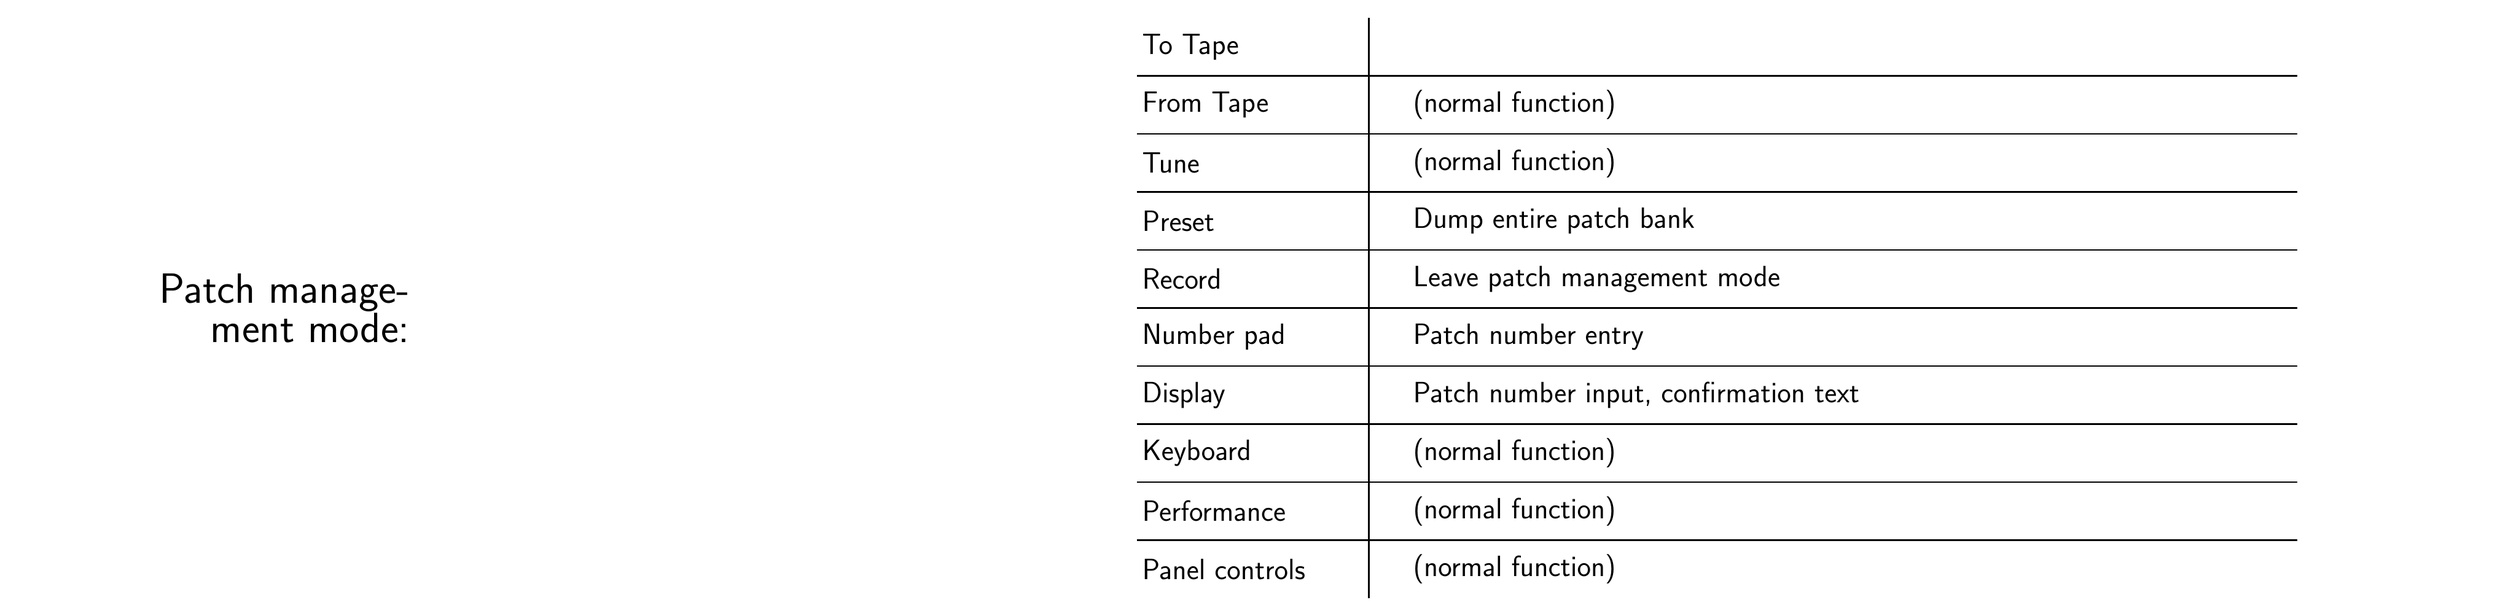
\begin{tikzpicture}[scale=0.8]
  \node[font=\fontsize{26}{22}\selectfont, align=right, outer sep=0.5mm, anchor = west, text width=8cm] at (0cm,12cm) {Patch management mode:};
    \upperbuttons{13cm,7cm}{P}{P}

    \node[font=\fontsize{18}{22}\selectfont, align=left, outer sep=0.0mm, anchor = west, text width=8cm] at (29cm,5.25cm) {Panel controls};
    \node[font=\fontsize{18}{22}\selectfont, align=left, outer sep=0.0mm, anchor = west, text width=22cm] at (36cm,5.25cm) {(normal function)};
    \draw[line width=1pt]++(29cm,6cm)--++(30cm,0cm);     
    \node[font=\fontsize{18}{22}\selectfont, align=left, outer sep=0.0mm, anchor = west, text width=8cm] at (29cm,6.75cm) {Performance};
    \node[font=\fontsize{18}{22}\selectfont, align=left, outer sep=0.0mm, anchor = west, text width=22cm] at (36cm,6.75cm) {(normal function)};
    \draw[line width=1pt]++(29cm,7.5cm)--++(30cm,0cm);     
    \node[font=\fontsize{18}{22}\selectfont, align=left, outer sep=0.0mm, anchor = west, text width=8cm] at (29cm,8.25cm) {Keyboard};
    \node[font=\fontsize{18}{22}\selectfont, align=left, outer sep=0.0mm, anchor = west, text width=22cm] at (36cm,8.25cm) {(normal function)};
    \draw[line width=1pt]++(29cm,9cm)--++(30cm,0cm);     
    \node[font=\fontsize{18}{22}\selectfont, align=left, outer sep=0.0mm, anchor = west, text width=8cm] at (29cm,9.75cm) {Display};
    \node[font=\fontsize{18}{22}\selectfont, align=left, outer sep=0.0mm, anchor = west, text width=22cm] at (36cm,9.75cm) {Patch number input, confirmation text};
    \draw[line width=1pt]++(29cm,10.5cm)--++(30cm,0cm);     
    \node[font=\fontsize{18}{22}\selectfont, align=left, outer sep=0.0mm, anchor = west, text width=8cm] at (29cm,11.25cm) {Number pad};
    \node[font=\fontsize{18}{22}\selectfont, align=left, outer sep=0.0mm, anchor = west, text width=22cm] at (36cm,11.25cm) {Patch number entry};
    \draw[line width=1pt]++(29cm,12cm)--++(30cm,0cm);     
    \node[font=\fontsize{18}{22}\selectfont, align=left, outer sep=0.0mm, anchor = west, text width=8cm] at (29cm,12.75cm) {Record};
    \node[font=\fontsize{18}{22}\selectfont, align=left, outer sep=0.0mm, anchor = west, text width=22cm] at (36cm,12.75cm) {Leave patch management mode};
    \draw[line width=1pt]++(29cm,13.5cm)--++(30cm,0cm);  
    \node[font=\fontsize{18}{22}\selectfont, align=left, outer sep=0.0mm, anchor = west, text width=8cm] at (29cm,14.25cm) {Preset};
    \node[font=\fontsize{18}{22}\selectfont, align=left, outer sep=0.0mm, anchor = west, text width=22cm] at (36cm,14.25cm) {Dump entire patch bank};
    \draw[line width=1pt]++(29cm,15cm)--++(30cm,0cm);  
    \node[font=\fontsize{18}{22}\selectfont, align=left, outer sep=0.0mm, anchor = west, text width=8cm] at (29cm,15.75cm) {Tune};
    \node[font=\fontsize{18}{22}\selectfont, align=left, outer sep=0.0mm, anchor = west, text width=22cm] at (36cm,15.75cm) {(normal function)};
    \draw[line width=1pt]++(29cm,16.5cm)--++(30cm,0cm);  
    \node[font=\fontsize{18}{22}\selectfont, align=left, outer sep=0.0mm, anchor = west, text width=8cm] at (29cm,17.25cm) {From Tape};
    \node[font=\fontsize{18}{22}\selectfont, align=left, outer sep=0.0mm, anchor = west, text width=22cm] at (36cm,17.25cm) {(normal function)};
    \draw[line width=1pt]++(29cm,18cm)--++(30cm,0cm);  
    \node[font=\fontsize{18}{22}\selectfont, align=left, outer sep=0.0mm, anchor = west, text width=8cm] at (29cm,18.75cm) {To Tape};
    \node[font=\fontsize{18}{22}\selectfont, align=left, outer sep=0.0mm, anchor = west, text width=22cm] at (36cm,18.75cm) {};
    
    \draw[line width=1pt]++(35cm,4.5cm)--++(0cm,15cm);  

  \end{tikzpicture}
}


\textbf{Dumping the patch library as SysEx} 

To dump the entire patch bank press the \preset button. The screen will scroll a confirmation message. Note, however, that only valid presets are exported. Any unused patch slots are skipped.

\textbf{Dumping single patches as SysEx} 

To dump a single patch in patch management mode simply enter the patch number on the number pad. Note, that if there is no valid patch data stored in the selected patch slot, the entry will be accepted but there will be no dump.

Note: the Prophet-600 also supports MIDI dump requests. When sending a SysEx patch request for a particular patch number to the Prophet-600 you will receive the corresponding single SysEx back (on the specified MIDI send channel) provided the specified patch number is between 0 and 99 and a valid patch is stored at this number. This can be done in all modes at any time, not just in \patchmgmt.

\textbf{Loading patches} 

Loading MIDI SysEx patches to storage is done by sending the patch SysEx containing the data to the Prophet-600 in \patchmgmt. Each patch contains a patch number. If the patch number is  between 0 and 99 the data will stored in that patch slot overwriting the existing stored patch. Therefore, loading a SysEx patch library will overwrite the entire library stored on the Prophet-600 when \patchmgmt is activated. When a patch has been loaded to storage the number of the patch number is shown on the display.

In normal \presetmode patch MIDI is only loaded into the active control values as described above. In \livemode incoming patch MIDI SysEx is ignored. Requiring \patchmgmt to be activated for MIDI-to-storage operations protects your patches from accidental overwrite. Still, it is always advisable to regularly archive patches in SysEx files outside the instrument.


\section{Scaling adjustment}\label{maintenance}

The Prophet 600 can be started in maintenance mode by shortening "TP301 SCALE" and powering up. 

In this mode the display shows the current oscillator/filter (A1..A6,B1..B6,F1..F6) and a value that needs to be made close or equal to zero by tweaking the corresponding adjustable.

Press 1 to go to next oscillator/filter, press 2 to go the previous one.

When done, turn off the synth and unshort TP301, next start will be in normal mode.


\section{SysEx firmware upgrade}\label{fwupgrade}

For a firmware upgrade in a Prophet 600 with an original Z80 processor please refer to the modification instructions \cite{modinstructions}. The following section is for owners of a modified Prophet 600 with Teensy board and a prior version of the GliGli upgrade installed. If modifying a Prophet 600 for the time one may directly flash the Teensy board with software version 2.2. It is not necessary to first install a lesser version and then upgrade.

Firmware upgrades are provided as MIDI SysEx files (*.syx) \footnote{They are also provided as *.hex files for USB transfer to the Teensy board.}. In order to perform the upgrade follow to step below.

\begin{enumerate}
  \setlength\itemsep{0cm}
  \item Switch off the instrument
  \item Switch on the instrument while holding the buttons \textbf{To Tape} and \textbf{From Tape} down. The display should show an "U" for upgrade on the left digit.
  \item Send the firmware SysEx file to the instrument. This process takes a while. The display shows a spinning segment. Once the process is completed, the display shows an "S" for success. If the upgrade ends with “E” for error on the display, the upgrade has failed and the upgrade procedure must be repeated until it succeeds. It is not recommended to start the instrument in normal mode after a failed upgrade.
  \item Switch the instrument off and on again. The scrolled welcome message should state the version "GliGli's P600 Upgrade Version \textit{<version>}"
\end{enumerate}

Users are recommended to follow the MIDI SysEx part of the modification instructions \cite{modinstructions}. In particular, the "Delay between buffers" and the "delay after F7" should be set to at least 250ms.

The settings and preset parameters are left unchanged by the upgrade, provided the previously installed version is one for which backward compatibility is supported. This applies to the following versions:

\begin{itemize}
  \setlength\itemsep{0cm}
  \item Version 2.0
  \item Version 2.1 Release Candidate 3 (not officially released)
  \item Version 2.2  
\end{itemize} 

Downgrading versions is possible but preservation of settings and preset parameters is not guaranteed in that case.

\end{flowtext}

\chapter{Reference}

\section{Patch parameter overview}\label{patchref}

\footnotesize
\renewcommand{\arraystretch}{1.3}
\begin{tabular}{ p{2cm}|p{3cm}|p{6cm}|p{6cm}|p{6cm}} 
   Number & Group & \makebox{1st press} & \makebox{2nd press} & \makebox{3rd press}\\ \hline
  0 & Speed & \makebox{Seq/Arp Speed} \linebreak \textit{numeric 0...98} & &  \\ \hline
  1 & LFO & \makebox{LFO Shape} \linebreak \textit{tri-square, sin-random, saw-noise} & \makebox{LFO Target} \linebreak \textit{A\&B, A, B, A \& B \& VCA } &  \makebox{LFO Sync} \linebreak \textit{off, 1, 2, 3, 4, 5, 6, 8} \\ \hline
  2 & \makebox{Vibrato} & \makebox{Vibrato Speed} \linebreak \textit{numeric 0...98} & \makebox{Vibrato Amount} \linebreak \textit{numeric 0...98} & \makebox{Vibrato Target} \linebreak \textit{VCO, VCA} \\   \hline
  3 & \makebox{Modulation Wheel} & \makebox{Modulation Target} \linebreak \textit{LFO, vibrato} & \makebox{Modulation Delay} \linebreak \textit{numeric 0...98} & \makebox{Moduation Wheel Range} \linebreak \textit{touch, soft, high, full} \\ \hline
  4 & \makebox{Configuration} & \makebox{OSC Pitch Mode} \linebreak \textit{free, semi-tones, octaves} & \makebox{External Voltage} \linebreak \textit{numeric 0...98} & \makebox{Sync Bug} \linebreak \textit{on, off} \\ \hline
  5 & Envelope & \makebox{Filter Envelope Shape} \linebreak \textit{fast-lin, fast-exp, slo-lin, slo-exp}  & \makebox{2nd Envelope Shape} \linebreak \textit{fast-lin, fast-exp, slo-lin, slo-exp} &
  \makebox{Envelope Routing} \linebreak \textit{std, poly-amp, poly, gate}\\ \hline
  6 & Bender & \makebox{Bend Target} \linebreak \textit{off, VCO, VCF, amp} & \makebox{Bend Range}  \linebreak \textit{2nd, 3rd, 5th, octave} &  \\ \hline
  7 & \makebox{Play Mode} & \makebox{Note Priority} \linebreak \textit{last, low, high} & \makebox{Voice Assigner} \linebreak \textit{first, cycle} & Glide\footnote{\glide is only available in \textit{GliGli} panel layout} \linebreak \textit{numeric 0...98}  \\ \hline
  8 & \makebox{Oscillator} & Detune \linebreak \textit{numeric 0...98}  &   \makebox{Vintage (Spread)} \linebreak \textit{numeric 0...98} & \makebox{Drive}\footnote{\drive is only available in \textit{SCI} panel layout} \linebreak \textit{numeric 0...98} \\ \hline
  9 & \makebox{Touch Sensitivity} & \makebox{Amplitude Velocity} \linebreak \textit{numeric 0...98}  & \makebox{Filter Velocity} \linebreak \textit{numeric 0...98} &  \\
  
\end{tabular}

\normalsize


\section{Settings parameter overview}\label{settingsref}

\footnotesize
\renewcommand{\arraystretch}{1.6}
\begin{tabular}{ p{2cm}|p{4cm}|p{6cm}|p{6cm}} 
   \textbf{Number} & \textbf{Purpose} & \makebox{\textbf{1st press}} & \makebox{\textbf{Repeated press}} \\
 \hline
  0 & \makebox{MIDI mode} & \makebox{Show current selected voice status} & \makebox{Toggle MIDI mode} \linebreak \textit{local on, local off}  \\
 \hline
  1 & \makebox{MIDI Receive} & \makebox{Show current MIDI receive channel} & \makebox{Cycle through channels} \linebreak \textit{OMNI, Ch1 ... Ch16} \\
 \hline
  2 & \makebox{MIDI Send} & \makebox{Show current MIDI send channel} & \makebox{Cycle through channels} \linebreak \textit{Ch1 ... Ch16} \\
 \hline
  3 & \makebox{Bender Calibration} & \makebox{Activate calibration mode} & \makebox{Confirmation} \\
 \hline
  4 & \makebox{Voice Selection} & \makebox{Show current selected voice} & \makebox{Cycle through voices} \linebreak \textit{1 ... 6} \\
 \hline
  5 & \makebox{Voice Deactivate} & \makebox{Show current selected voice status} & \makebox{Toggle voice status} \linebreak \textit{on, off} \\
 \hline
  6 & \makebox{Panel Layout} & \makebox{Show current selected panel layout} & \makebox{Toggle panel layout} \linebreak \textit{GliGli, SCI} \\
 \hline
  7 & \makebox{Unused} & & \\
 \hline
  8 & \makebox{Clock Sync} & \makebox{Show current clock sync} & \makebox{Cycle through sync types} \linebreak \textit{internal, MIDI, tape}  \\
 \hline
  9 & \makebox{VCF limit} & \makebox{Show current setting} & \makebox{Cycle through settings} \linebreak \textit{on, off}  \\
 \hline
  Preset & \makebox{Default Patch} & \makebox{Activate default patch load} & \makebox{Confirmation} \\
 \hline
  Tune & \makebox{Per Note Tuning} & \makebox{Activate per note tuning} & \makebox{Deactivate/save per note tuning} \\
 \hline
  Record & \makebox{MIDI Patch Receive Mode} & \makebox{Activate MIDI patch receive mode} & \makebox{End MIDI patch receive mode} \\
  \end{tabular}
\normalsize


\section{MIDI control implementation}\label{midiimplenentation}

Two types of MIDI events are implemented in the ,upgraded Prophet-600:

\begin{itemize}
  \setlength\itemsep{0cm}
  \item MIDI CC Continuous parameters: value resolution of 0-16383 using 2 CCs (fine and coarse), or value resolution of 0-127 using only the coarse one
  \item MIDI CC Stepped parameters: 0-127, variable number of steps. They work by dividing the 0-127 range in as many zones as there are choices for the parameter. E.g.: "Unison" is an on-off parameter and therefore has s choices. In this case it is \textit{off} for 0-63 and it is \textbf{on} for 64-127.
  \item Performance events (note events, pitch bend)
  \item Real time events
  \item SysEx (for different purposes)
\end{itemize}

The Prophet-600 receives Continuous Controllers (CC) which correspond to patch parameters in \presetmode only. 

\section{MIDI CC Patch Parameters} 

\footnotesize
\renewcommand{\arraystretch}{1.3}

\begin{longtable}[l]{ p{5cm}|p{2cm}|p{1.5cm}|p{1.5cm}|p{5cm}|p{2cm}|p{1cm}} 
\textbf{Continuous Parameter} & \textbf{Type} & \textbf{CC Coarse} & \textbf{CC Fine} & \textbf{Stepped Parameter} & \textbf{Type} & \textbf{CC} \\ \hline
\endfirsthead
\textbf{Continuous Parameter} & \textbf{Type} & \textbf{CC Coarse} & \textbf{CC Fine} & \textbf{Stepped Parameter} & \textbf{Type} & \textbf{CC} \\ \hline
\endhead 
Osc A Frequency & Continuous & 16 & 80 & Osc A Saw & Stepped & 48 \\ \hline
Osc A Volume & Continuous & 17 & 81 & Osc A Triangle & Stepped & 49 \\ \hline
Osc A Pulse Width & Continuous & 18 & 82 & Osc A Square & Stepped & 50 \\ \hline
Osc B Frequency & Continuous & 19 & 83 & Osc B Saw & Stepped & 51 \\ \hline
Osc B Volume & Continuous & 20 & 84 & Osc B Triangle & Stepped & 52 \\ \hline
Osc B Pulse Width & Continuous & 21 & 85 & Osc B Sqr & Stepped & 53 \\ \hline
Osc B Fine & Continuous & 22 & 86 & Sync & Stepped & 54 \\ \hline
Cutoff & Continuous & 23 & 87 & Poly Mod Oscillator A Destination & Stepped & 55 \\ \hline
Resonance & Continuous & 24 & 88 & Poly Mod Filter Destination & Stepped & 56 \\ \hline
Filter Envelope Amount & Continuous & 25 & 89 & LFO Shape & Stepped & 57 \\ \hline
Filter Release  &  Continuous  & 26 & 90 &  LFO Targets  &  (see \ref{lfotarget})  &  59 \\ \hline
Filter Sustain  &  Continuous  & 27 & 91 &  Keyboard Filter Tracking  &  Stepped  &  60 \\ \hline
Filter Decay  &  Continuous  & 28 & 92 &  Filter Envelope Shape  &  Stepped  &  61 \\ \hline
Filter Attack  &  Continuous  & 29 & 93 &  Filter Envelope Fast/Slow  &  Stepped  &  62 \\ \hline
2nd Release  &  Continuous  & 30 & 94 &  2nd Envelope Shape  &  Stepped  &  63 \\ \hline
2nd Sustain  &  Continuous  & 31 & 95 &  Unison  &  Stepped  &  65 \\ \hline
2nd Decay  &  Continuous  & 32 & 96 &  Assigner Priority Mode  &  Stepped  &  66 \\ \hline
2nd Attack  &  Continuous  & 33 & 97 &  Bender Range (semitones)  &  (see \ref{bendsemi})  &  67 \\ \hline
Poly Mod Filter Amount  &  Continuous  & 34 & 98 &  Bender Target  &  Stepped  &  68 \\ \hline
Poly Mod Osc B Amount  &  Continuous  & 35 & 99 &  Mod Wheel Range  &  Stepped  &  69 \\ \hline
LFO Frequency  &  Continuous  & 36 & 100 &  Osc pitch mode  &  Stepped  &  70 \\ \hline
LFO Amount  &  Continuous  & 37 & 101 &  Mod Wheel Target  &  Stepped  &  71 \\ \hline
Glide  &  Continuous  & 38 & 102 &  Vibrato Target  &  Stepped  &  72 \\ \hline
Amp Velocity  &  Continuous  & 39 & 103 &   2nd Envelope Fast/Slow  &  Stepped  &  73 \\ \hline
Filter Velocity  &  Continuous  & 40 & 104 &  Sync Bug  &  Stepped  &  74 \\ \hline
Modulation delay  &  Continuous  & 41 & 105 &  Voice Assign  &  Stepped  &  75 \\ \hline
Vibrato frequency  &  Continuous  & 42 & 106 &  Envelope Routing  &  Stepped  &  76 \\ \hline
Vibrato amount  &  Continuous  & 43 & 107 &  LFO Sync  &  Stepped  &  77 \\ \hline
Unison detune  &  Continuous  & 44 & 108 &    &    &   \\ \hline
External CV amount  &  Continuous  & 46 & 110 &  &  &   \\ \hline 
Vintage / Spread  &  Continuous  & 47 & 111 &  &  &   \\ \hline 
 
\end{longtable}

\normalsize

\section{MIDI CC Settings}

Unlike MIDI CC event for patch parameters, which are only applied in \presetmode, the following MIDI CC controls are always applied. 

\renewcommand{\arraystretch}{1.3}

\begin{longtable}[l]{ p{6cm}|p{2.5cm}|p{1.5cm}|p{2cm}|p{7cm}} 
\textbf{Parameter} & \textbf{Type} & \textbf{CC} & \textbf{CC Fine} & \textbf{Comment on CC value} \\ \hline
Toggle Live/Preset Mode & Stepped & 0 & & 0 = live mode, 1 = preset mode \\ \hline
Mod Wheel & Continuous & 1 & & \\ \hline
Master Volume & Continuous & 7 & & \\ \hline
Sequencer / arpeggiator clock & Continuous & 45 & 109 & \\ \hline
Hold Pedal & Stepped & 64 & & 0 = release, >0 = hold/latch\\ \hline
All Sound Off & Stepped & 120 & & 127 = sound off\\ \hline
Local On/Off & Stepped & 122 & & <=63 = local on, >63 = local off \\ \hline
All Notes Off & Stepped & 123 & & 0 = all notes off\\ \hline
\end{longtable}

\section{Special parameters and technical information}

\subsection*{LFO Targets (MIDI CC 59)}\label{lfotarget}

MIDI CC 59 LFO Target is a stepped parameter. It combines the effects of the LFO panel controls (separate switches for targeting the VCO, the filter cutoff and the pulse width) with the additional patch parameter which provides further options (targeting VCA, targeting oscillators A and B separately). These options are encoded bitwise in the parameter as shown in the table below. Each bit represents \textit{off} or \textit{on} for the respective switch/option. 

\renewcommand{\arraystretch}{1.3}

\begin{longtable}[l]{p{1.2cm}|p{2cm}|p{4cm}} 
\textbf{Bit} & \textbf{Value} & \textbf{Function} \\ \hline
\endfirsthead
\textbf{Bit} & \textbf{Value} & \textbf{Function} \\ \hline
\endhead 
1 & 1 & VCO \\ \hline 
2 & 2 & Filter \\ \hline 
3 & 4 & VCA \\ \hline 
4 & 8 & Pulse Width \\ \hline 
5 & 16 & Only A \\ \hline 
6 & 32& Only B \\ \hline 
\end{longtable}


Example: if the filter and the VCO targets are active and the modulation is restricted to oscillator B then the parameter takes the following value:

LFO Targets (MIDI CC 59) = 1 (VCO) + 2 (filter) + 32 (only B) = 35

Note that the same parameter encoding is also used in the patch MIDI SysEx implementation. Not all combinations of bits are possible (at least when edited on the unit) and meaningful. Some can only be achieved using MIDI CC or SysEx.
\begin{itemize}
  \item The options "Only A" and "Only B" only affect the targets VCO and pulse width (VCA and filter are shared by the two oscillators)
  \item When editing a patch from the Prophet-600 it is impossible to set bits 5 and 6 simultaneously. Technically the effect of setting both bits (by sending such a patch configuration to the Prophet-600 via SysEx or MIDI CC) would be that VCO and pulse width are modulated for neither oscillator even if those targets are activated. 
  \item When editing a patch from the Prophet-600 it is impossible to activate the VCA target and at the same time restrict the VCO or pulse width modulation to one of the oscillators. This is purely due to user interface restrictions. It is perfectly possible to choose this option using MIDI CC or SysEx. 
\end{itemize}


\subsection*{Bender Range (semitones) (MIDI CC 67)}\label{bendsemi}

The MIDI CC 67 parameter which controls the bender range behaves like a stepped parameter. However, unlike other stepped parameters whose value corresponds to the index of the selected option, the value of the bend range parameter contains the actual number of semitones. The allowed values and the corresponding option names as shown on the Prophet-600 display are as follows. 

\renewcommand{\arraystretch}{1.3}

\begin{longtable}[l]{p{1.2cm}|p{4cm}} 
\textbf{Value} & \textbf{Text} \\ \hline
\endfirsthead
\textbf{Value} & \textbf{Text} \\ \hline
\endhead 
2 & 2nd \\ \hline 
3 & 3rd \\ \hline 
5 & 5th \\ \hline 
8 & Octave \\ \hline 
\end{longtable}

No other values are allowed.

\subsection*{Changes in MIDI CC implementation from version 2.1 RC3 to \version}

The following MIDI CC have been changed.

\begin{itemize}
  \item For the filter envelope release and decay and the 2nd envelope release and decay the time value range has been rescaled for the \textit{linear} envelope shape. This was an unavoidable side effect of changing the strictly linear shapes to linear shapes with soft tails. The exponential envelopes are unaffected.
  \item The \lfofreq has been totally rescaled. The stepped frequency range parameter has been omitted and the value range of the \lfofreq dial now covers the entire frequency range. However, the dial to frequency relation has also been changed from linear to exponential, making it much softer at low settings. Consequently, the MIDI CC support for the LFO frequency range (up to firmware version 2.1 RC3) has been omitted. In order to avoid potential conflicts with MIDI tools developed for firmware versions 2.0 and 2.1 RC3, the legacy MIDI CC 58 has not been re-designated. MIDI CC 58 is ignored.
  \item The value to frequency relation for the \vibspeed has been changed from linear to exponential.   
  \item The \modwheelrange has been reconfigured with new value which also produce different wheel actions.
\end{itemize}


\normalsize


\chapter{Technical reference for the GliGli upgrade}

\section{Clock cycle}

(this nees to be done)

\section{Settings storage}

(this nees to be done)

\section{Patch storage}

(this nees to be done)

\chapter{Troubleshooting}

(this nees to be done)

\begin{thebibliography}{50} 

\bibitem{gligli}GliGli Projects Page, http://gliglisynth.blogspot.com/
\bibitem{curtis}Curtis Electro Music on Webarchive, https://web.archive.org/web/20130502132536/http://curtiselectromusic.com/Customers\_and\_Instruments.html
\bibitem{versiontwo}GliGli upgrade release 2.0,  https://gligli.github.io/p600fw/
\bibitem{modinstructions} Prophet600 Modification Instructions
\bibitem{projectsite} Project Site: http://gligli.github.io/p600fw/
\bibitem{repository} Repository: https://github.com/gligli/p600fw/
\bibitem{teensy}Teensy Site: http://www.pjrc.com/teensy/index.html
\bibitem{p600siownersmanual}Prophet 600 Owner's Manual, Sequential Circuits
\bibitem{p600siservicemanual} Prophet 600 Service Manual, Sequential Circuits

\end{thebibliography}

\end{document}
